% this file is called up by thesis.tex
% content in this file will be fed into the main document
\chapter{Código/Manuales/Publicaciones}
% top level followed by section, subsection


%%%%%%%%%%%%%%%%%%%%%%%%%%%%%%%%%%%%%%%%%%%%%%%%%%%%%%%%%%%%%%%%%%
\section{Simulaciones con XFLR5}
\label{Simulaciones con XFLR5}
XFLR5 es un software de código abierto ampliamente utilizado para el análisis aerodinámico y el diseño de aeronaves.
%
Fue desarrollado principalmente por Mark Drela, un destacado ingeniero aeroespacial y profesor en el Instituto de Tecnología de Massachusetts (MIT). Su experiencia en aerodinámica y diseño de aeronaves fue fundamental para la creación de esta herramienta.
%
El desarrollo de XFLR5 comenzó en la década de 1990, lo que significa que ha estado en desarrollo y evolución durante varias décadas. Esto ha permitido que la herramienta madure y se convierta en una opción confiable para los ingenieros y diseñadores de aeronaves.
%
 XFLR5 se distribuye bajo una licencia de código abierto, lo que significa que el software es gratuito y su código fuente está disponible para que cualquiera lo examine, modifique y distribuya. Esto ha fomentado una comunidad activa de usuarios y desarrolladores que contribuyen a su mejora continua. Se especializa en el análisis aerodinámico de aeronaves y planeadores. Ofrece características clave como el cálculo de coeficientes aerodinámicos, la generación de curvas de polar, la simulación de vuelo, la optimización de perfiles aerodinámicos y más. 
\begin{figure}[h]
    \centering
    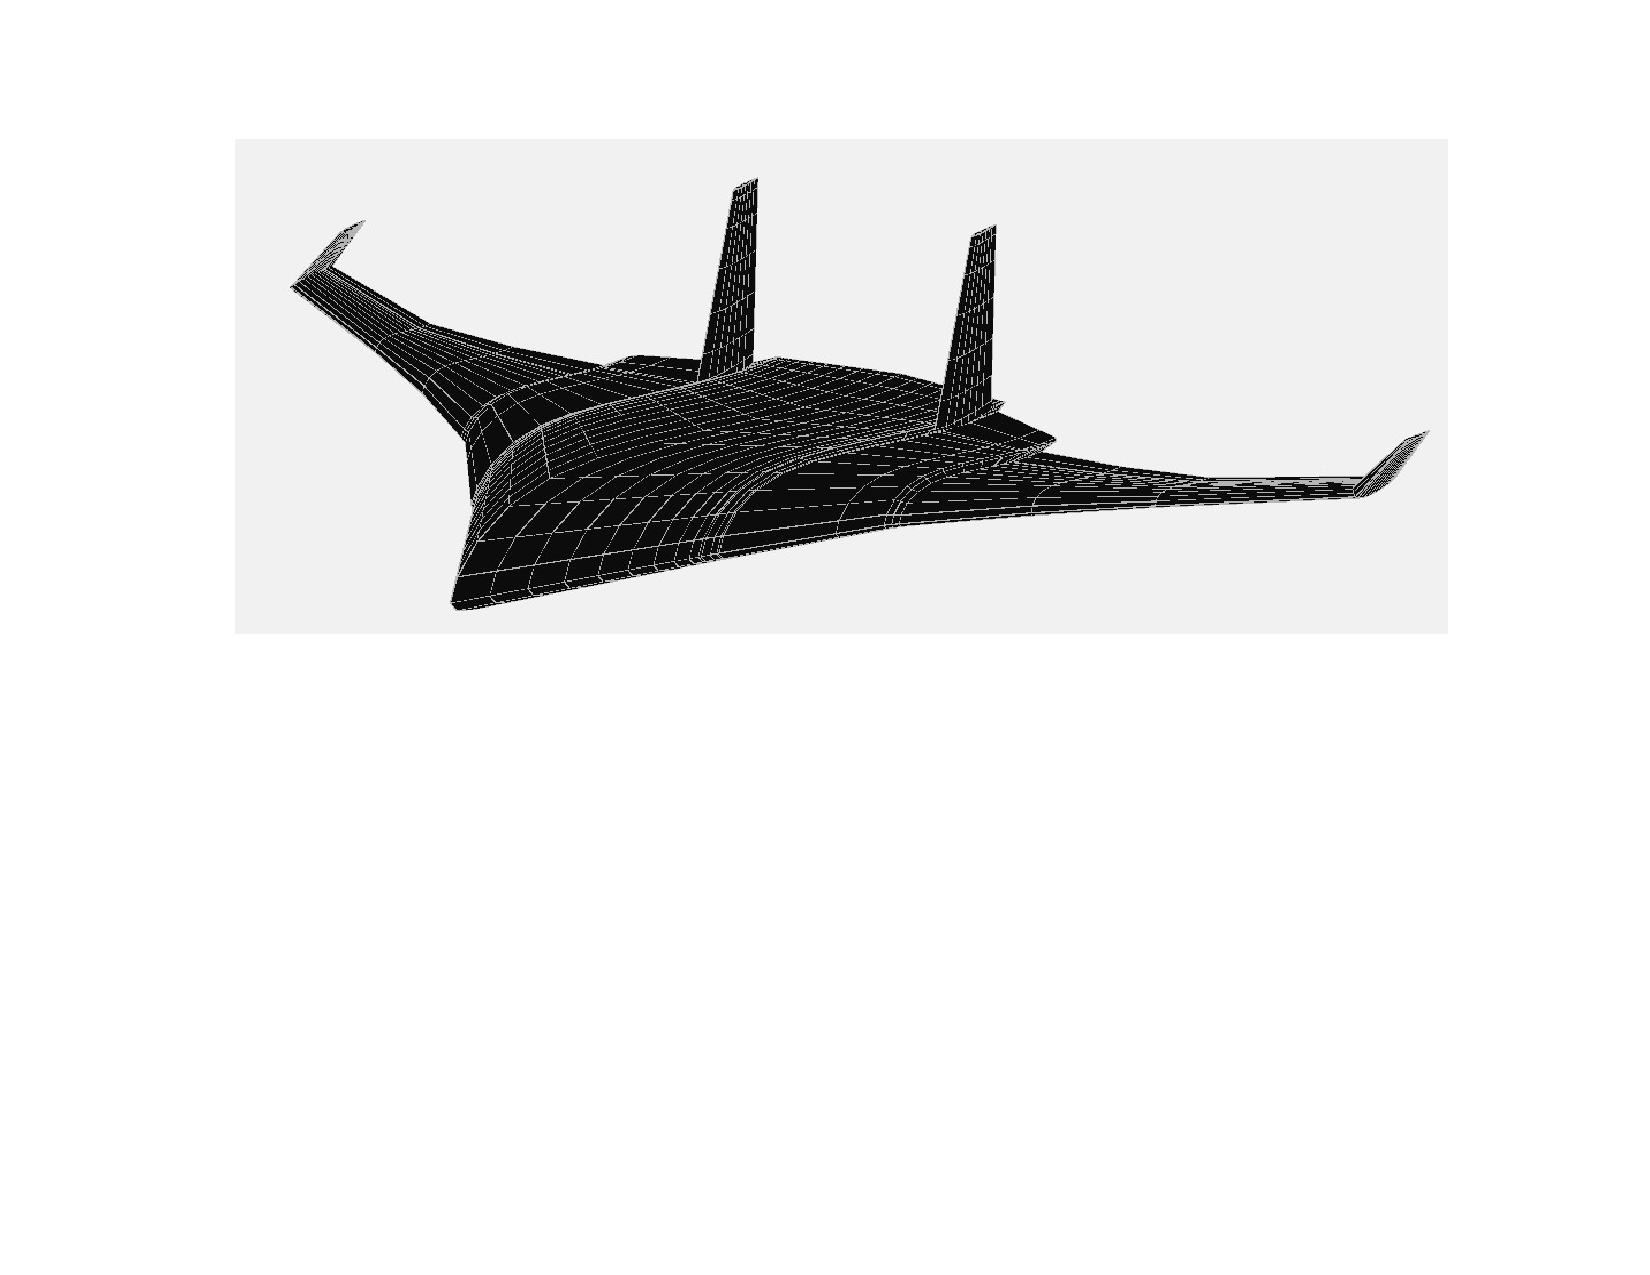
\includegraphics[scale=0.65]{Capitulo3/figs/paneles ehekatl_cropped.pdf}          
    \caption{Malla de paneles para simulaciones aerodinámicas}
    \label{Malla de paneles para simulaciones aerodinámicas}
\end{figure}

  Su historia y su enfoque en el código abierto lo convierten en una herramienta valiosa para la comunidad de ingeniería aeroespacial.
%
En la figura \ref{Malla de paneles para simulaciones aerodinámicas}, observamos a EHEKATL BWB G-33 y la malla considerada en paneles.  En la tabla \ref{EHEKATL BWB G-33 ficha geometrica} habíamos mencionado que establecios 644 paneles para nuestro mallado. 
XFLR5 cuenta con tres métodos numéricos para la solución del análisis aerodinámico. 
\begin{itemize}
    \item \textbf{Teoría de la línea de sustentación} Es un modelo simplificado que se utiliza para comprender y analizar la aerodinámica de un ala, especialmente en el contexto de alas finitas (alas con una envergadura limitada en lugar de alas infinitas). puedes modelar la aerodinámica de un ala dividiéndola en segmentos, cada uno tratado como un perfil aerodinámico separado. Estos segmentos están conectados a lo largo de la envergadura del ala, formando una línea continua o curva conocida como "línea de sustentación". Cada segmento genera sustentación de manera individual en función de su ángulo de ataque local y las características del perfil aerodinámico.La Teoría de la Línea de Sustentación en XFLR5 te permite aproximar la sustentación y la resistencia inducida de un ala finita. Es una herramienta valiosa para analizar el rendimiento de alas de aeronaves en el mundo real
    \item \textbf{Vórtices de herradura} Un vórtice de herradura es un patrón de flujo complejo que se produce cerca de las puntas de las alas de una aeronave u otros cuerpos sustentadores. Cuando una aeronave genera sustentación, crea una diferencia de presión entre las superficies superior e inferior de sus alas. Esta diferencia de presión induce el flujo de aire desde la región de alta presión debajo del ala hacia la región de baja presión arriba. Cerca de las puntas de las alas, este flujo se enrolla y forma un patrón de vórtice que se asemeja a una herradura. Este vórtice de herradura es un contribuyente significativo a la resistencia inducida.
 Comprender la presencia y el comportamiento de los vórtices de herradura es crucial para el diseño de aeronaves y la optimización aerodinámica. Los ingenieros buscan minimizar la intensidad de estos vórtices para reducir la resistencia y mejorar la eficiencia.
    \item \textbf{Vórtice anular} XFLR5 no modela directamente vórtices anulares, ya que están típicamente asociados con turbulencia de estela y la interacción de aeronaves en escenarios del mundo real. Sin embargo, el software puede proporcionar información sobre el comportamiento del flujo cerca de las puntas de las alas y los bordes de fuga que pueden contribuir a la formación de vórtices anulares. 
Aunque XFLR5 no simula explícitamente vórtices anulares, puede ayudarte a comprender los patrones de flujo y las condiciones que podrían llevar a su formación. Este conocimiento puede orientarte en el diseño de alas y aeronaves para minimizar el impacto de la turbulencia de estela.
\item  \textbf{Paneles 3D} En el contexto de XFLR5 y el análisis aerodinámico de aeronaves, los "paneles 3D" se refieren a una técnica numérica que descompone la superficie del ala y la aeronave en una serie de elementos bidimensionales (paneles) que representan partes de la superficie. 
Estos paneles 3D pueden considerarse como superficies planas que aproximadamente siguen la forma del ala y la aeronave en tres dimensiones.
Cada panel 3D tiene propiedades aerodinámicas asociadas, como ángulo de ataque, curvatura, posición en el espacio y coeficientes aerodinámicos.
XFLR5 utiliza esta descomposición de paneles 3D para calcular las fuerzas y momentos aerodinámicos actuando sobre la aeronave en función de los parámetros de vuelo y los ajustes de control. Los métodos de paneles 3D son una forma eficiente de realizar análisis aerodinámicos detallados de una aeronave, teniendo en cuenta la geometría tridimensional y las condiciones de vuelo.
\end{itemize}

El análisis de estabilidad de XFLR5 se basa en la solución de las ecuaciones de movimiento lineales de una aeronave en respuesta de pequeñas perturbaciones. Cuando se realiza el análisis de estabilidad y control para así también obtener los coeficientes de las ACS, la principal limitación es que en esta caso la simulación no considera el arrastre viscoso. 
Podemos definir las siguientes \textbf{limitaciones} en el uso de XFLR5:
%
1)  Modelos de Flujo Potencial: XFLR5 se basa en modelos de flujo potencial, lo que significa que no resuelve las ecuaciones de Navier-Stokes completas, sino que se basa en simplificaciones. Esto lo hace adecuado para análisis de alas y perfiles aerodinámicos a velocidades subsónicas y transónicas, pero no es adecuado para el análisis de flujos supersónicos o hipersónicos.
%
2) Aproximación de Pequeñas Perturbaciones: XFLR5 asume que las perturbaciones inducidas por la aeronave en el flujo son pequeñas, lo que es válido para la mayoría de las aplicaciones aeronáuticas convencionales. Sin embargo, no es adecuado para el análisis de aeronaves de alta velocidad o alta maniobrabilidad, como aviones de combate supersónicos.
%
3) Simplificaciones en la Geometría: El software utiliza una serie de simplificaciones geométricas, como perfiles alares bidimensionales y modelos de alas rectas. Esto puede limitar su capacidad para modelar geometrías complejas o efectos de ala variable. 
%
4) Limitaciones en las Condiciones de Operación: XFLR5 es más adecuado para el análisis de condiciones de operación subsónicas y transónicas. No es la herramienta adecuada para el análisis de aeronaves hipersónicas o cohetes.
%
5) Sensibilidad a los Datos de Entrada: La precisión de las simulaciones en XFLR5 puede depender en gran medida de la calidad de los datos de entrada, como los perfiles aerodinámicos y las propiedades del flujo. Los resultados pueden variar si los datos no son precisos o si falta información importante.
%
6) Capacidades de Análisis Limitadas: Aunque es útil para el análisis de alas y perfiles aerodinámicos, XFLR5 no tiene las capacidades de análisis más avanzadas que ofrecen herramientas de Dinámica de Fluidos Computacional (CFD) completas. No puede capturar efectos de flujo tridimensional complejo, efectos de estabilidad y control avanzados o interacciones aire-aire complejas.
%
7) No es una Herramienta de Diseño Final: XFLR5 es útil para el diseño conceptual y análisis preliminar, pero no está diseñado para el diseño y análisis detallado de aeronaves a nivel de ingeniería final. Es una herramienta valiosa para la fase inicial de diseño, pero los diseñadores suelen recurrir a herramientas más especializadas para análisis y validación posteriores. 
%
8) Precisión en el arrastre viscoso:  XFLR5 se basa principalmente en métodos de análisis potencial y, por lo tanto, es más adecuado para calcular la sustentación y el arrastre inducido (asociado a la sustentación). Sin embargo, tiene limitaciones en el cálculo preciso del arrastre viscoso, que es el arrastre relacionado con la fricción del flujo viscoso sobre la superficie de un ala. XFLR5 utiliza un modelo simplificado de arrastre viscoso que asume que el flujo es incompresible y que la capa límite es delgada. Esto puede llevar a inexactitudes en el cálculo del arrastre en ciertos casos, especialmente en configuraciones donde la capa límite es significativa o en perfiles aerodinámicos con alta velocidad. Está diseñado principalmente para el análisis bidimensional y, aunque puede manejar configuraciones 3D, no es tan preciso para casos altamente tridimensionales o con efectos 3D complejos. Las configuraciones de alas en forma de cuerda de golondrina o alas con geometrías muy irregulares pueden presentar desafíos.Para mejorar la precisión en el cálculo del arrastre viscoso, XFLR5 puede depender de datos experimentales o coeficientes de arrastre proporcionados por el usuario. Esto significa que la precisión del cálculo del arrastre viscoso puede depender de la calidad y disponibilidad de datos experimentales.

%%%%%%%%%%%%%%%%%%%%%%%%%%%%%%%%%%%%%%%%%%%%%%%%%%%%%%%%%%%%%%%%%%
\section{Modelado del EHEKATL BWB con Control de Empuje Vectorial}
\label{modelado TVC}

El \textbf{Control  del Vector de Empuje } a través de dos servo-mecanismos de una tobera articulada genera momentos de cabeceo $\delta_{\theta}$ y guiñada $\delta_{\psi}$,  con un momento de brazo de acuerdo con

\begin{equation}
\label{eq: momento brazo del vector de empuje}
    l_T = x_{cg} - x_T
\end{equation}


dónde $x_{cg}$ es el centro de gravedad de la aeronave, donde actúan las fuerzas externas, y $x_T$ es el eje axial del TVC respecto al origen del sistema de referencia de propulsión y control de empuje vectorial.  


\begin{figure}[h]
\centering
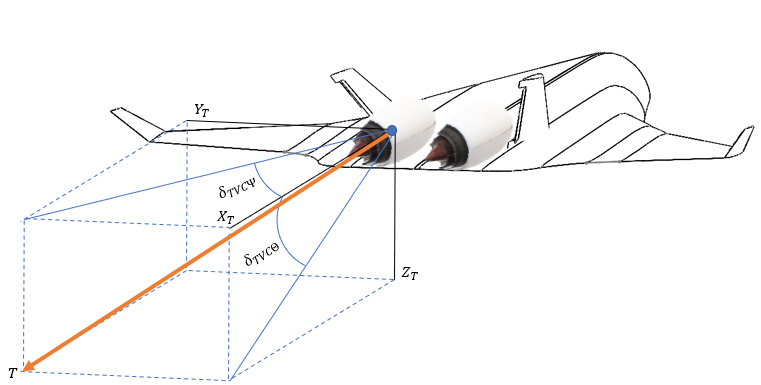
\includegraphics[scale=0.7]{Capitulo3/figs/4 13.png}
\caption{Fuerzas y momentos del control de empuje vectorial }
\label{fig: fuerzas y momentos del control de empuje vectorial}
\end{figure}


Ahora vamos a descomponer las fuerzas y momentos para identificar la aplicación y la ecuación del vector de empuje en cada eje. 

\begin{figure}[h]
\centering
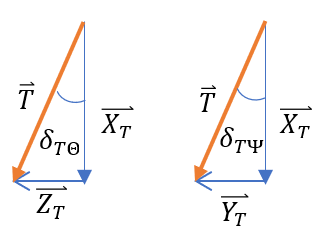
\includegraphics[scale=0.8]{Capitulo3/figs/4 14.png}
\caption{Componentes del control del empuje vectorial }
\label{fig: componentes del control de empuje vectorial}
\end{figure}

La transformación que generan los momentos del TVC $\delta_{TVC \Theta}, \delta_{TVC \Psi}$ es igual a los momentos que se generan en el centro de gravedad de la aeronave $M_T, N_T$. 

Dada la deflexión de $\delta_{TVC \Theta}$ para el momento de cabeceo (primer triángulo de izquierda a derecha), mostrada en \ref{fig: componentes del control de empuje vectorial}, definimos los componentes del vector de empuje en el plano simétrico X-Z. 


\begin{equation}
    X_T = T C_{\delta_{T\Theta}}, \\
    Z_T = T S_{\delta_{T\Theta}}
\end{equation}

y el momento de cabeceo $M_T$ generado en la aeronave es 

\begin{equation}
    M_T = l_T Z_T
\end{equation}

Ahora definimos de manera similar la deflexión de $\delta_{TVC \Psi}$ para el momento de guiñada, de acuerdo con el segundo triángulo-rectángulo. 

\begin{equation}
    X_T = T C_{\delta_{T\Psi}}, \\
    Y_T = T S_{\delta_{T\Psi}}
\end{equation}

el momento de guiñada $N_T$ generado en la aeronave es 

\begin{equation}
    N_T = l_T Y_T
\end{equation}

Las ecuaciones que describen el comportamiento en cada eje se muestran a continuación

\begin{align}
    X_{T} &= P_T C_{\theta} C_{\psi} \\
    Y_{T} &= P_T  S_{\psi}  \\
    Z_{T} &= P_T  C_{\psi} S_{\theta} 
\end{align}

Entonces los componentes del control de empuje vectorial en los ejes cuerpo queda representado en las fuerzas lineales 
\begin{equation}
\begin{bmatrix}
X_{T} \\
Y_{T} \\
Z_{T}
\end{bmatrix}
=
T
\begin{bmatrix}
C_{\delta_{\Theta}} C_{\delta_{\Psi}} \\
S_{\delta_{\Psi}} \\
S_{\delta_{\Theta}}
\end{bmatrix}
\end{equation}

y en los momentos angulares como

\begin{equation}
\begin{bmatrix}
L_{T} \\
M_{T} \\
N_{T}
\end{bmatrix}
=
\begin{bmatrix}
0 \\
l_T Z_{T} \\
l_T Y_{T}
\end{bmatrix}
\end{equation}

De acuerdo con nuestra configuración EHEKATL BWB son dos motores los que actuarían sus toberas TVC, por lo que se tiene que considerar las variables de cada una, y entonces se establecen los momentos lineales

\begin{align}
    X_T &= T_{1} C_{\delta1_{\Theta}} C_{\delta1_{\Psi}} + T_{2} C_{\delta2_{\Theta}} C_{\delta2_{\Psi}} \\
    Y_T &= T_{1} S_{\delta1_{\Psi}} + T_{2} S_{\delta2_{\Psi}} \\
    Z_T &= T_{1} S_{\delta1_{\Theta}} + T_{2} S_{\delta2_{\Theta}}
\end{align}

y los momentos angulares

\begin{align}
    L_T &= 0 \\
    M_T &= l_T(T_1 Y_{T1} + T_2 Y_{T2}) \\
    N_T &= l_T(T_1 Z_{T1} + T_2 Z_{T2})
\end{align}

%%%%%%%%%%%%%%%%%%%%%%%%%%
\section{Modelado de términos de acoplamiento de estabilidad y control}

En el modelo acoplado no-lineal es posible representar las fuerzas de acoplamiento mediante derivadas de estabilidad, términos que no se desarrollan normalmente. 
Cuando tenemos los modelos desacoplados asumimos que los movimientos de guiñada y alabeo no producen ningún movimiento en cabeceo, y viceversa. 
Una de las áreas que suelen omitirse durante el modelado en la dinámica de vuelo es el modelado de las fuerzas de acoplamiento. Entre más de 20 derivadas acopladas, dos de ellas son las más importantes para representar los efectos de la dinámica lateral-direccional y longitudinal, son las derivadas de acoplamiento del ángulo de derrape $C_{D_{\beta}}$ y el ángulo de alabeo $C_{L_{\phi}}$. Podemos ser negligentes con el resto de derivadas y únicamente considerar estas dos. 
La razón por la cual estos dos coeficientes son suficientes para considerar el modelo acoplado no-lineal completo son las siguientes: 
Un movimiento longitudinal puro no tiene un efecto directo en la mecánica lateral-direccional, el principal efecto del movimiento direccional en la mecánica longitudinal es incrementar la fuerza axial (principalmente el arrastre), y por tanto reduce la velocidad longitudinal de la aeronave.

Por tanto el valor más significativo es de la derivada $C_{D_{\beta}}$.
El principal efecto del movimiento lateral en la mecánica longitudinal es la de reducir la fuerza normal (en otras palabras la fuerza de sustentación) de la aeronave. Por tanto, la principal derivada es $C_{L_{\phi}}$. 

Definidas las derivadas de acoplamiento y actualizando las fuerza axial y  la fuerza normal el modelado acoplado no-lineal obtenemos
\begin{gather}
    X = X_{\alpha} \alpha + X_{\dot \alpha}\dot \alpha + X_{u} u + X_{q} q + X_{\delta_{e}} \delta_{e} + X_{\beta} \beta \\
    Z = Z_{\alpha} \alpha + Z_{\dot \alpha}\dot \alpha + Z_{u} u + Z_{q} q + Z_{\delta_{e}} \delta_{e} + Z_{\phi} \phi
\end{gather}

y de acuerdo con \cite{Mohammad2020}. 

\begin{gather}
    X_{\beta} = (sign(\beta))q_{1}S_{vt}\frac{2}{\pi} \\
    Z_{\phi} = 0.1 mg (sign(\phi))
\end{gather}
Dónde la función signo es una convención de signos. 

Existen superficies de control aerodinámicas que son consideradas sobre-actuadas. Los \textbf{timon-elevador} y los \textbf{elevons}. 
El timon-elevador se usa particularmente cuando se tiene estabilizadores verticales en forma V, si ambas superficies van hacia la misma dirección, sea en un sentido o en otro generamos el momento de guiñada, si las superficies van en direcciones contrarias pero misma magnitud, podemos generar el momento de cabeceo. 
Los elevons son la principal propuesta para Ala-Integrada debido el cuantioso número de entradas de control en el borde de fuga. Si se mueven en la misma dirección y magnitud generamos cabeceo, si lo hacen en la misma magnitud pero diferente dirección generan el momento de alabeo. 
Gracias a la notación de \cite{Beard2012} podemos convertir los timones-elevadores y los elevons 

\textbf{timones-elevadores}
\begin{equation}
\begin{bmatrix}
\delta_{e} \\
\delta_{r}
\end{bmatrix}
=
\begin{bmatrix}
1 & 1 \\
-1 & 1 
\end{bmatrix}
\begin{bmatrix}
\delta_{rr} \\
\delta_{rl}
\end{bmatrix}
\end{equation}

\textbf{elevons}
\begin{equation}
\begin{bmatrix}
\delta_{e} \\
\delta_{a}
\end{bmatrix}
=
\begin{bmatrix}
1 & 1 \\
-1 & 1 
\end{bmatrix}
\begin{bmatrix}
\delta_{er} \\
\delta_{el}
\end{bmatrix}
\end{equation}


Finalmente, podemos declarar los términos de las fuerzas aerodinámicas

\begin{align}
    X_A &= X_{u}u + X_{\alpha}\alpha + X_{\dot \alpha}\dot \alpha + X_{q}q + X_{\beta} \beta \\
    Z_A &= Z_{u}u + Z_{\alpha}\alpha + Z_{\dot \alpha}\dot \alpha + Z_{q}q + Z_{\phi} \\
    Y_A &= Y_{p}p + Y_{r}r + Y_{\beta}\beta + Y_{\dot \beta}\dot \beta  \\
    L_A &= L_{p}p + L_{r}r + L_{\beta}\beta + L_{\dot \beta}\dot \beta \\
    M_A &= M_{u}u + M_{\alpha}\alpha + M_{\dot \alpha}\dot \alpha + M_{q}q  \\
    N_A &= N_{p}p + N_{r}r + N_{\beta}\beta + N_{\dot \beta}\dot \beta
\end{align}

Y los términos de las fuerzas de control

\begin{align}
    X_C &=  X_{\delta_{e}}\delta_{e} \\
    Z_C &=  Z_{\delta_{e}}\delta_{e} \\
    Y_C &=  Y_{\delta_{a}}\delta_{a} + Y_{\delta_{r}} \delta_{r}\\
    L_C &=  L_{\delta_{a}}\delta_{a} + L_{\delta_{r}} \delta_{r} \\
    M_C &=  M_{\delta_{e}}\delta_{e} \\
    N_C &=  N_{\delta_{a}}\delta_{a} + N_{\delta_{r}} \delta_{r}
\end{align}


En las fuerzas externas lineales aplicadas los términos del vector de velocidad del aire $X_{\alpha} \alpha, Y_{\beta} \beta$ suelen  emplearse transformando $ X_{w} w, Y_{v} v$ respectivamente. Se consideran los términos $ X_{\dot w} \dot w, Y_{\dot v} \dot v$ o $ X_{\dot \alpha} \dot \alpha, Y_{\dot \beta} \dot \beta$ según sea el caso, aunque en la revisión del estado-del-arte se menciona que estas derivadas suelen ser pequeñas comparadas con el resto de lo términos y podemos ser negligentes con ellas. 



%%%%%%%%%%%%%%%%%%%%%%%
\section{Linealización}
\label{linealizacion a}
Para nuestro proceso de linealización nos basamos principalmente en \cite{Etkin1996}, \cite{Lewis2016}, \cite{Schimdt1998}, \cite{USAF1988} y \cite{Mohammad2020}. 


En realidad el modelo no-lineal es quién aproxima al sistema físico real de la aeronave. Sin embargo, tratar con modelos no lineales no es una tarea sencilla. La linealización convierte  el modelo no-lineal considerando pequeñas desviaciones o perturbaciones desde el equilibrio. Por tanto, podemos decir que el proceso de linealización cancela o ignora las no-linealidades del sistema \cite{Mohammad2020}.
G. H. Bryan (1911) introdujo la idea de las perturbasciones en las fuerzas y los momentos respecto a un estado de equilibrio $trim$ como condición de vuelo, y esta aproximación es la más usada hasta ahora \cite{Cook2007}. 


Existen dos métodos básicos para el proceso de linealización: 
\begin{itemize}
    \item Linealización Jacobiana (Series de Taylor)
    \item Linealización por retroalimentación (dinámica inversa)
\end{itemize}

La \textbf{linealización Jacobiana} literalmente es negligente con las no-linealidades del modelo, mientras que la \textbf{linealización por retroalimentación} activamente suprime las no-linealidades \cite{Mohammad2020}.

Es bien reconocido que en una aeronave pueden cambiar las configuraciones de vuelo rápidamente (transición de ascenso a crucero, desaceleración desde el descenso hasta la aproximación, deflactar los \textit{}{flaps} y extender el tren de aterrizaje, etc.), el proceso de linealización debe ser considerado respecto a una condición de vuelo de fija \cite{Schimdt1998}. 
La linealización subsecuente de las ecuaciones de movimiento nos permite una determinación de comportamiento dinámico de amplitudes pequeñas de la aeronave alrededor de un punto de equilibrio o \textit{trim}. 
Algunas consideraciones importantes para el análisis de perturbación incluyen:

\begin{itemize}
    \item Los pequeños movimientos de la dinámica serán iniciados desde el vuelo a nivel del ala con los controles y la configuración del empuje de la aeronave en equilibrio, a esto se le conoce como \textbf{condición de vuelo de equilibrio estático}.
    \item El eje-cuerpo será alineado con el vector de velocidad inicial, y por mucho, será conocido como el eje-estabilidad de la aeronave.
\end{itemize}

Cualquier sistema de ecuaciones no lineales puede ser linealizado en un punto de equilibrio. La linealización es solamente válida en la vecindad del punto de equilibrio. 
El punto de equilibrio no tiene aceleración, es decir, la velocidad es constante. 
Algunas operaciones de vuelo en puntos de equilibrio son: 
\begin{itemize}
    \item Vuelo crucero con velocidad constante
    \item Ascenso con velocidad constante
    \item Vuelta con velocidad constante
\end{itemize}

El despegue y aterrizaje no tienen condiciones de equilibrio, dado que la velocidad del aire no es constante. El sistema lineal satisface la propiedad de superposición y homogeneidad. 

Un forma general de una ecuación lineal es $y=mx$, dónde $m$ es referido como la pendiente y es un número constante. 
Un término lineal tiene grado uno en la variable dependiente y su derivada. 
Una ecuación lineal consiste en una suma de términos lineales \cite{Mohammad2020}.  
La linealización entonces alrededor de un punto de equilibrio puede ser alcanzada de dos maneras:
\begin{itemize}
    \item Usando series de Taylor
    \item Substituyendo directamente
\end{itemize}

El procedimiento usual es asumir que las fuerzas y momentos aerodinámicos son dependientes en las variables de movimiento perturbadas y en sus derivadas únicamente.  

La serie de Taylor expresa una función de suma de cada una de las variables de movimiento o su derivada. 
Dado que las variables de movimmiento son $u,v,w$ y $p,q,r$, cada uno de estos términos sería una función $f_i$, y ejemplificando en el eje axial con el término $X$ obtendríamos: 

\begin{equation}
    X = X_{e} + (\frac{\partial X}{\partial u}u+\frac{\partial^2 X}{\partial^2 u}\frac{u^2}{2!}+\frac{\partial^3 X}{\partial^3 u}\frac{u^3}{3!} + ...)
\end{equation}

y esta serie aplica para cada función de variable de movimiento, lineal y angular, en su primer derivada y de orden superior, dónde el primer término es una constante $X_{e}$. 

Dado que la teoría de las pequeñas perturbaciones considera estas perturbaciones dentro de la vencidad del punto de equilibrio, el movimiento de las variables es pequeño, y para todos los casos prácticos sólo el término de primer orden en cada una de las series es significativo. El único término de orden superior que suele considerarse es $ \dot \alpha$ o $\dot w$. En muchas ocasiones el valor de este término es pequeño comparada con los de primer orden y por simplicidad podría omitirse. 

Entonces definiríamos las derivadas de estabilidad del sistema lineal tal que 

\begin{align}
    X_a &= X_u u + X_{w}w + X_q q + X_{G}G \\
    Y_a &= Y_{v}v + Y_{p}p + Y_{r}r + Y_{G}G \\
    Z_a &= Z_u u + Z_{w}w + Z_q q + Z_{G}G  \\
    L_a &= L_{v}v + L_{p}p + L_{r} \\
    M_a &= M_u u + M_{w}w + M_q q \\
    N_a &= N_{v}v + N_{p}p + N_{r}r
\end{align}

y los términos de las derivadas de control quedarían definidos como
\begin{align}
\label{eq: entradas de control lineal}
X_c &= \textcolor{RoyalBlue}{X_{\delta_T} \delta_T}  + \textcolor{RoyalBlue}{X_{\delta_{e1}} \delta_{e1}} + \textcolor{RoyalBlue}{X_{\delta_{e2}} \delta_{e2}}  \\
Y_c &= \textcolor{RoyalBlue}{Y_{\delta_T} \delta_T}  + \textcolor{RoyalBlue}{Y_{\delta_{a1}\delta_{a1}}} + \textcolor{RoyalBlue}{Y_{\delta_{a2}\delta_{a2}}} + \textcolor{RoyalBlue}{Y_{\delta_{r}}\delta_{r}} \\
Z_c &= \textcolor{RoyalBlue}{Z_{\delta_T} \delta_T}  + \textcolor{RoyalBlue}{Z_{\delta_{e1}} \delta_{e1}} + \textcolor{RoyalBlue}{Z_{\delta_{e2}} \delta_{e2}}  \\
L_c &= \textcolor{RoyalBlue}{L_{\delta_{a1}\delta_{a1}}} + \textcolor{RoyalBlue}{L_{\delta_{a2}\delta_{a2}}} + \textcolor{RoyalBlue}{L_{\delta_{r}}\delta_{r}} \\
M_c &= \textcolor{RoyalBlue}{M_{\delta_{e1}} \delta_{e1}} + \textcolor{RoyalBlue}{M_{\delta_{e2}} \delta_{e2}} \\
N_c &= \textcolor{RoyalBlue}{N_{\delta_{a1}\delta_{a1}}} + \textcolor{RoyalBlue}{N_{\delta_{a2}\delta_{a2}}} + \textcolor{RoyalBlue}{N_{\delta_{r}}\delta_{r}}
\end{align}



La \textbf{técnica directa} está basada en la teoría de las pequeñas perturbaciones, donde substituyes todas las variables independientes, por ejemplo X con dos términos $X_0,\Delta X(t)$, el de la condición inicial de equilibrio y el término de la perturbación. 

Dado que asumimos las perturbaciones en $x$ pequeñas implica tener solamente los términos lineales. 

Las variables angulares las vamos a simplificar también con la teoría de las pequeñas perturbaciones, dónde el $sin(x)$ se normaliza igual a x, y el $cos(x)$ es igual a uno.  

Antes de la linealización, el conjunto de las seis ecuaciones de movimiento acopladas aparecerá como:

\begin{gather}
    X_0 + \Delta X(t) - mg sin\theta = m(\dot u + qw - rv) \\
    Y_0 + \Delta Y(t) + mg cos\theta sin\phi = m (\dot v + ru - pw) \\
    Z_0 + \Delta Z(t) + mg cos\theta cos \phi = m ( \dot w + pv - qu) \\
    L_0 + \Delta L(t) = I_x \dot p - I_xz \dot r + (I_z - I_y)pr - I_xz pq \\
    M_0 + \Delta M(t) = I_y \dot q + (I_x - I_z) pr + I_xz (p^2 - r^2) \\
    N_0 + \Delta N(t) = I_z \dot r - I_xz \dot p + (I_y - I_x)pq + I_xz qr
\end{gather}


De una manera semejante a las declaraciones de fuerzas y momentos, la linealización de las variables de estado dependientes del tiempo comenzará con una definición de los valores de equilibrio iniciales más los términos de pequeñas perturbaciones.

\begin{gather}
    u = u_0 + u(t) \\
    v = v_0 + v(t) = v(t) \\
    w = w_0 + w(t) = w(t) \\
    p = p_0 + p(t) = p(t) \\
    q = q_0 + q(t) = q(t)  \\
    r = r_0 + r(t) = r(t) \\
    \theta = \theta_0 + \theta(t) \\
    \phi = \phi_0 + \phi(t) = \phi(t) 
\end{gather}

La condición inicial considerada para el movimiento inicial desde el vuelo a nivel del ala con el eje-cuerpo correspondiente al eje-estabilidad de la aeronave permite la eliminación de los términos $v_0, w_0, p_0, q_0, r_0, \phi_0$ y se considera $u_0 = V_0$.

En el tiempo cero, cuando el movimiento de las pequeñas perturbaciones está por comenzar, la relación de las ecuaciones anteriores se simplifica de acuerdo con las condiciones de equilibrio estático en las fuerzas y momentos de la aeronave.

\begin{gather}
    X_0 - mg sin\theta_0 = 0 \\
    Y_0 = 0; (\phi_0) \\
    Z_0 + mg cos\theta_0 = 0 \\
    L_0 = M_0 = N_0 = 0
\end{gather}

De acuerdo con las condiciones de equilibrio estático, el eje $X$ tiene una condición inicial dado que $u$ y $\theta_0$ son las componentes en este eje que pueden tener un valor inicial distinto de cero, lo que al estar trabajando en el plano simétrico $X-Z$, la componente inicial en el eje Z también sería distinto de cero y proporcional al eje $X$. El término correspondiente a la fuerza aerodinámica en el eje Y es cero, dado que se considera el vuelo a nivel del ala y el ángulo $\phi_0=0$. Esto genera que en las componentes del peso tengamos en cuenta que $sin \phi_0 = 0$ y por tanto el efecto del peso no tiene presencia en el eje $Y$, y por lado $cos \phi_0 = 1$ , lo que deja el término de $cos \theta_0$ para la componente del peso en el eje $Z$ y en función del ángulo de cabeceo. 

Todos los momentos se consideran cero para está condición de vuelo en equilibrio estático. 

La relación de fuerzas envuelve términos trigonométricos que pueden ser linealizados usando las consideraciones de los ángulos para las pequeñas perturbaciones. 

El \textit{teorema de la suma y diferencia de ángulos} establece la relación para la suma de dos ángulos, como es el caso en la teoría de las pequeñas perturbaciones dado el ángulo de condición inicial y el ángulo considerando la fuerza aerodinámica. 

\begin{gather}
    sin(\theta_0 + \Delta \theta) = sin \theta_0 cos \Delta \theta + cos \theta_0 sin \Delta \theta \doteqdot sin\theta_0 + \Delta \theta cos \theta_0 \\
    cos(\theta_0 + \Delta \theta) = cos \theta_0 cos \Delta \theta - sin \theta_0 sin \Delta \theta \doteqdot cos\theta_0 - \Delta \theta sin \theta_0
\end{gather}

Entonces, en resumen:

\begin{gather}
    sin\Theta = sin \Theta_0 + cos\Theta_0 \theta(t) 
\end{gather} 
para $\theta(t) << 1$, y
\begin{gather}
    sin\Phi = \phi(t)
\end{gather}
para $\phi_0 = 0$ y $\phi(t) << 1$
\begin{gather}
    cos \Phi = 1
\end{gather}

La demostración del teorema \textit{la suma y diferencia de ángulos} se muestra en el capítulo de \textit{apéndices}.

Entonces las ecuaciones linealizadas quedarían de la siguiente manera


\begin{gather}
    X_0 + \Delta X(t) + X_c - mg = m(\dot u + q_0 w + q w_0 - r_0 v - r v_0) \\
    Y_0 + \Delta L(t) Y_c + mg = m (\dot v + r_0 u + r u_0 - p_0 w - p w_0) \\
    Z_0 + \Delta Z(t) + Z_c + mg = m ( \dot w + p_0 v + p v_0 - q_0 u - q u_0) \\
    L_0 + \Delta L(t) = I_x \dot p + (I_z - I_y)(q_0 r + q r_0) \\
    M_0 + \Delta M(t) = I_y \dot q + (I_x - I_z) (p_0 r + p r_0) \\
    N_0 + \Delta N(t) = I_z \dot r + (I_y - I_x)(p q_0 + p_0 q)
\end{gather}

y obtendríamos 

\begin{gather}
    \dot u  = \frac{1}{m}(X_0 + \Delta X(t) + X_c) - g - (q_0 w + q w_0 - r_0 v - r v_0) \\
    \dot v = \frac{1}{m}(Y_0 + \Delta Y(t) + Y_c) + g -( r_0 u + r u_0 - p_0 w - p w_0) \\
    \dot w = \frac{1}{m}(Z_0 + \Delta Z(t) + Z_c) + g -( p_0 v + p v_0 - q_0 u - q u_0) \\
    \dot p = \frac{1}{I_x}(L_0 + \Delta L(t) + L_c) - (I_z - I_y)(q_0 r + q r_0) \\
    \dot q = \frac{1}{I_y}(M_0 + \Delta M(t) + M_c) - (I_x - I_z) (p_0 r + p r_0) \\
    \dot r = \frac{1}{I_z}N_0 + \Delta N(t) + N_c) - (I_y - I_x)(p q_0 + p_0 q)
\end{gather}

y si consideramos el sistema de referencia de ejes viento, recordemos que 
\begin{gather}
    \dot V  = \frac{1}{mV}(X_0 + \Delta X(t) + X_c) - \frac{g}{V} - (q_0 \alpha + q \alpha_0 - r_0 \beta - r \beta_0) \\
    \dot \beta = \frac{1}{mV}(Y_0 + \Delta L(t) Y_c) + \frac{g}{V} -( r_0 u + r V_0 - p_0 \alpha - p \alpha_0) \\
    \dot \alpha = \frac{1}{mV}(Z_0 + \Delta Z(t) + Z_c) + \frac{g}{V} -( p_0 \beta + p \beta_0 - \alpha_0 V - \alpha V_0) \\
\end{gather}


%%%%%%%%%%%%%%%%%%%%%%%%%%%%%%%%%%%%%%%%%%%%%%%
\textbf{Modelo Dinámico Lineal Longitudinal - 3GDL}\\
En el desacople longitudinal consideramos únicamente las perturbaciones en el plano simétrico x-z
\begin{align}
    X_0 + \Delta X(t) + X_c - mg &= m(\dot u + q_0 w + q w_0) \\
    Z_0 + \Delta Z(t) + Z_c + mg &= m ( \dot w + q_0 u - q u_0) \\
    M_0 + \Delta M(t) &= I_y \dot q
\end{align}

dónde los términos $X_0,Z_0, M_0$ representan la condición de equilibrio y los términos $\Delta X(t),\Delta Z(t), \Delta M(t)$ las perturbaciones del sistema. A partir de este criterio podemos simplificar la nomenclatura sabiendo que los términos $X,Z,M$ representan las perturbaciones del sistema a partir del punto de equilibrio. Desarrollando los términos de fuerzas y momentos aplicados tenemos que

\begin{gather}
    X_u u + X_w w + X_q q + \textcolor{RoyalBlue}{X_c} - mg = m(\dot u + q_0 w + q w_0) \\
    Z_u u + Z_w w + Z_q q + \textcolor{RoyalBlue}{Z_c} + mg = m ( \dot w + q_0 u - q u_0) \\
    M_u u + M_w w + M_q q + \textcolor{RoyalBlue}{M_c} = I_y \dot q
\end{gather}

dónde las entradas de control consideradas son

\begin{equation}
    \textcolor{RoyalBlue}{X_c = X_{\delta_{T}} + X_{\delta_e1} \delta_e1 + X_{\delta_e2} \delta_e2}
\end{equation}

despejando las derivadas $\dot{u}, \dot{w},\dot{q},\dot{\theta}$ se obtiene

\begin{align}
    \dot u &=\frac{1}{m}(X_u u + X_w w + X_q q + \textcolor{RoyalBlue}{X_c}) - g -q w_0  \\
    \dot w &= \frac{1}{m}(Z_u u + Z_w w + Z_q q + \textcolor{RoyalBlue}{Z_c}) + g + q u_0 \\
    \dot q &= \frac{1}{I_y}(M_u u + M_w w + M_q q + \textcolor{RoyalBlue}{M_c}) \\  
    \dot \theta &= q
\end{align}

y considerando que la aeronave está en vuelo a nivel entonces

\begin{equation}
    \theta_{0} = w_0 = 0
\end{equation}

se puede simplificar la ecuación de la dinámica lineal longitudinal en su forma más simple

\begin{align}
\label{lineal longitudinal cuerpo}
    \dot u &=\frac{1}{m}(X_u u + X_w w + X_q q + \textcolor{RoyalBlue}{X_c}) - g \\
    \dot w &= \frac{1}{m}(Z_u u + Z_w w + (Z_q + mu_0) q + \textcolor{RoyalBlue}{Z_c}) + g \\
    \dot q &= \frac{1}{I_y}(M_u u + M_w w + M_q q + \textcolor{RoyalBlue}{M_c}) \\  
    \dot \theta &= q
\label{lineal longitudinal cuerpo 1}
\end{align}

de igual forma se puede escribir la dinámica en función de las variables de estado del ángulo de ataque y de la trayectoria de vuelo


\begin{align}
    \dot u &=\frac{1}{mV}(X_u u + X_\alpha \alpha + X_q q + \textcolor{RoyalBlue}{X_c}) - \frac{g}{V} \\
    \dot \alpha &= \frac{1}{mV}(Z_u u + Z_\alpha \alpha + (Z_q + mu_0) q + \textcolor{RoyalBlue}{Z_c}) + \frac{g}{V} \\
    \dot q &= \frac{1}{I_y}(M_u u + M_\alpha \alpha + M_q q + \textcolor{RoyalBlue}{M_c}) \\  
    \dot \theta &= q
\end{align}

\begin{align}
    \dot u &=\frac{1}{mV}(X_u u + X_\alpha \alpha + X_q q + \textcolor{RoyalBlue}{X_c}) - \frac{g}{V} \\
    \dot \gamma &= -\frac{1}{mV}(Z_u u + Z_\alpha \alpha + (Z_q + mu_0) q + \textcolor{RoyalBlue}{Z_c}) - \frac{g}{V} \\
    \dot q &= \frac{1}{I_y}(M_u u + M_\alpha \alpha + M_q q + \textcolor{RoyalBlue}{M_c}) \\  
    \dot \alpha &= q - \dot \gamma
\end{align}

%%%%%%%%%%%%%%%%%%%%%%%%%%%%%%%%%%%%%%%%%%%%%
\textbf{Modelo Dinámico Lineal Lateral-Direccional - 3 GDL}


La dinámica lineal lateral-direccional de tres grados de libertad se desacopla a continuación


\begin{gather}
    Y_0 + \Delta L(t) Y_c + mg = m (\dot v + r_0 u + r u_0 - p_0 w - p w_0) \\
    L_0 + \Delta L(t) = I_x \dot p + (I_z - I_y)(q_0 r + q r_0) \\
    N_0 + \Delta N(t) = I_z \dot r + (I_y - I_x)(p q_0 + p_0 q)
\end{gather}

considerando el mismo criterio de nomenclatura dónde se parte de una condición de equilibrio y únicamente consideramos los términos como peturbaciones del sistema, los términos dimensionales de las derivadas parciales de estabilidad y control serían

\begin{gather}
    Y_\beta \beta + Y_q q + Y_r r + Y_c + mg = m (\dot v + r u_0 - p w_0) \\
    L_\beta \beta + L_q q + L_r r + L_c = I_x \dot p \\
    N_\beta \beta + N_q q + N_r r + N_c = I_z \dot r
\end{gather}

dónde las entradas de control son

\begin{equation}
    \textcolor{RoyalBlue}{Y_c = Y_{\delta_{a1}} \delta_{a1} + Y_{\delta_{a2}} \delta_{a2} + Y_{\delta_{r}} \delta_{r}}
\end{equation}

Despejando las derivadas de estado y tomando en consideración \cite{Schimdt1998} para los valores de los coeficientes dimensionales. Simulando con estos coeficientes obtuvimos un mejor comportamiento en las señales de las entradas de control. 

\begin{gather}
    \dot v = \frac{1}{m}(Y_\beta \beta + Y_q q + Y_r r + Y_c) + g - r u_0 \\
    \dot p = \frac{1}{I_x}(L_\beta' \beta + L_q' q + L_r' r + L_c') \\
    \dot r = \frac{1}{I_z}(N_\beta' \beta + N_q' q + N_r' r + N_c') \\
    \dot \phi = p
\end{gather}

y expresando en términos aerodinámicos, y recordando que $u_0 = V_0 = V$

\begin{gather}
    \dot \beta = \frac{1}{mV}(Y_\beta \beta + Y_q q + (Y_r - mu_0) r + Y_c) + \frac{g}{V} \\
    \dot p = \frac{1}{I_x}(L_\beta' \beta + L_q' q + L_r' r + L_c') \\
    \dot r = \frac{1}{I_z}(N_\beta' \beta + N_q' q + N_r' r + N_c') \\
    \dot \phi = p
\end{gather}





%%%%%%%%%%%%%%%%%%%%%%%%%%%%%%%%%%%%%%%%%%%%%%%%%%%%%%%%%%%%%%%%%%%%%%%%%%%
\section{Superficie Alar y Potencia Requerida}
\label{superficie alar y potencia requerida}

\textit{Matching plot} es un enfoque gráfico que permite determinar la \textbf{superficie alar} y la \textbf{potencia requerida}. 
\begin{itemize}
    \item[] Objetivos de diseño en \textit{Matching plot}
    \item Área de referencia ($S_{ref}$)
    \item Empuje requerido ($T$) o Potencia requerida ($P$)
\end{itemize}
%
Las curvas en \textit{matching plot} son la razón de empuje-peso o poder de carga (eje de abcisas) en función de la carga alar (eje de ordenadas). 

La \textbf{carga alar $\frac{W}{S}$} es la razón entre el peso de la aeronave y el área o superficie de referencia. La carga alar indica cuanta carga soporta la superficie alar por unidad de área. 

La \textbf{razón de empuje-peso $\frac{T}{W}$} es la relación que indica cuánto empuje puede generar la aeronave en relación con su peso total. 
Cuanto mayor sea la relación empuje-peso, más capacidad tendrá la aeronave para acelerar y mantener el vuelo en situaciones como despegue, ascenso o maniobras. 

La \textbf{razón de peso-empuje $\frac{W}{T}$} es la relación inversa de $\frac{T}{W}$. Indica cuánto peso debe soportar la aeronave por cada unidad de empuje que produce. Cuanto menor sea la relación de peso-empuje, más eficiente será la aeronave, ya que necesitará menos empuje para soportar su peso. 

La \textbf{razón de potencia-peso $\frac{P}{W}$} es la relación que indica cuanta potencia está disponible para mover una unidad de peso. Una mayor relación $\frac{P}{W}$ es deseable, ya que la aeronave indica una mayor capacidad de aceleración y rendimiento. 

La \textbf{razón de peso-potencia $\frac{W}{P}$} es la relación inversa de $\frac{P}{W}$. Indica cuánto peso se debe soportar por cada unidad de potencia disponible. Cuanto menor sea $\frac{P}{W}$, más eficiente será la aeronave, ya que necesitará menos potencia para soportar su peso. 


La razón de empuje-peso $\frac{T}{W}$ suele emplearse para determinar el empuje de motores jet,  turbofan o turbojet. 
La razón de peso-potencia $\frac{W}{P}$ suele emplearse en aeronaves propulsadas por hélices o propelas (\textit{turboprop o motores piston}).

\begin{itemize}
    \item Velocidad de entrada en pérdida $ (\frac{W}{P} )_{V_s} = f_1 (\frac{W}{S}, V_s)$
    \item Velocidad máxima $ (\frac{W}{P} )_{V_{max}} = f_2 (\frac{W}{S}, V_{max})$
    \item Régimen de ascenso  $ (\frac{W}{P} )_{ROC} = f_2 (\frac{W}{S}, ROC)$
    \item Largo de pista de despegue $ (\frac{W}{P} )_{S_{TO}} = f_3 (\frac{W}{S}, S_{TO})$
    \item Techo de servicio absoluto $ (\frac{W}{P} )_{ceiling_{a}} = f_3 (\frac{W}{S}, h_a)$
    \item Techo de servicio crucero $ (\frac{W}{P} )_{ceiling_{c}} = f_3 (\frac{W}{S}, h_c)$
\end{itemize}

La velocidad de pérdida $V_s$, la velocidad máxima $V_{max}$, el régimen de ascenso $ROC$, el largo de la pista de despegue $S_{TO}$, el techo de servicio absoluto $ceiling_a$ y el techo de servicio en crucero $ceiling_c$ son los requerimientos de desempeño de la aeronave mostrados en curvas en la gráfica \textit{matching plot} de acuerdo con el empuje o potencia requerida en función de la carga alar. 
%
Las ecuaciones (funciones de cada variable) se consideran de \cite{Mohammad2020} y \cite{Sadraey2013}. 

\begin{table}[!h]
    \caption{Requerimientos de la Misión de Vuelo}
    \centering
    \begin{tabular}{|c|c|c|}
    \hline
    \multicolumn{3}{|c|}{\textbf{Parámetros de Entrada para Matching Plot} } \\
    \hline
    \multicolumn{3}{|c|}{\textbf{Requerimientos de Misión de Vuelo}} \\
    \hline
    Rango de vuelo & $12, 060 m$ & $39, 566.92 ft$ \\
    \hline
    Velocidad de entrada en pérdida & $19 m/s$ & $62.33 ft/s$  \\
    \hline
    Velocidad de despegue &  $22.8 m/s$ & $74.8 ft/s$ \\
    \hline
    Velocidad crucero & $27 m/s$ & $88.58 ft/s$ \\
    \hline
    Velocidad máxima & $35.1 m/s$ & $115.15 ft/s$ \\
    \hline
    Altitud & $2, 400 m$ & $7, 874 ft$\\
    \hline
    Largo de pista para despegue & $30 m$ & $3.28 ft$ \\
    \hline
    Regimen de ascenso & $2.5 m/s$ & $8.2 ft/s$ \\
    \hline
    Techo de servicio absoluto & $120 m$ & $393.7 ft$ \\
    \hline
    Techo se servicio crucero & $90 m$ & $295.27 ft$ \\
    \hline
    \multicolumn{3}{|c|}{\textbf{Coeficientes Aerodinámicos}} \\
    \hline
    Coeficiente de levantamiento $C_L$ & \multicolumn{2}{|c|}{$0.2$} \\
    \hline
    Coeficiente de arrastre $C_D$ & \multicolumn{2}{|c|}{$0.013$}  \\
    \hline
    Coeficiente de arrastre en despegue $C_{D0}$ & \multicolumn{2}{|c|}{$0.025$} \\
    \hline
    Coeficiente de levantamiento max. $C_{L_{max}}$ & \multicolumn{2}{|c|}{$0.48$} \\
    \hline
    Coeficiente de arrastre max. $C_{D_{max}}$ & \multicolumn{2}{|c|}{$0.028$}  \\
    \hline
    \multicolumn{3}{|c|}{\textbf{Geometría}} \\
    \hline
    Área de referencia & $1.4m^2$ & $15.06 ft^2$ \\
    \hline
    Relación de Aspecto & \multicolumn{2}{|c|}{$3.9$} \\
    \hline
    \end{tabular}
    \label{Requerimientos de la misión de vuelo}
\end{table}
%%%%%%%%%%%%%%%%%%%
%\begin{table}[h]
%    \centering
%    \begin{tabular}{|c|c|c|}
%    \hline
%    \multicolumn{3}{|c|}{\textbf{Parámetros de operación para Matching Plot}} \\
%    \hline
%    \multicolumn{3}{|c|}{Desempeño aerodinámico} \\
%    \hline
%    Coeficiente de levantamiento $C_L$ & \multicolumn{2}{|c|}{$0.2$} \\
%    \hline
%    Coeficiente de arrastre $C_D$ & \multicolumn{2}{|c|}{$0.013$}  \\
%    \hline
%    Coeficiente de arrastre en despegue $C_{D0}$ & \multicolumn{2}{|c|}{$0.025$} \\
%    \hline
%    Coeficiente de levantamiento max. $C_{L_{max}}$ & \multicolumn{2}{|c|}{$0.48$} \\
%    \hline
%    Coeficiente de arrastre max. $C_{D_{max}}$ & \multicolumn{2}{|c|}{$0.028$}  \\
%    \hline
%    \end{tabular}
%    \caption{Desempeño aerodinámico}
%    \label{desempeño aerodinamico}
%\end{table}
%%%%%%%%%%%%%%%%%%%%%%%%
%\begin{table}[h]
%    \centering
%    \begin{tabular}{|c|c|c|}
%    \hline
%    \multicolumn{3}{|c|}{\textbf{Parámetros de operación para Matching Plot} } \\
%    \hline
%    \multicolumn{3}{|c|}{Geometría del sistemas aéreo no tripulado} \\
%    \hline
%    Área de referencia & $1.3 m^2$ & $3.22 ft^2$ \\
%    \hline
    %Relación de Aspecto & \multicolumn{2}{|c|}{$4.6$} \\
    %\hline
    %\end{tabular}
    %\caption{Geometría de referencia del sistema aéreo ni tripulado para matching %plot}
%    \label{geometria para matching plot}
%\end{table}

%
Los requerimientos de la misión de vuelo, coeficientes aerodinámicos y parámetros geométricos de EHEKATL BWB para desarrollar \textit{Matching Plot} y seleccionar el punto de diseño se muestran en la tabla \ref{Requerimientos de la misión de vuelo}.
%
Se desarrolló un código en PYTHON que muestra las curvas de \textit{Matching plot} en base a los requerimientos de entrada para que el usuario pueda deteminar el punto de diseño.
%
El código muestra los resultados para ambos sistemas de propulsión (motores a reacción y de hélices) y en ambos sistemas unidades (Inglés e Internacional). 
%
\begin{table}[!h]
    \caption{Sistema de Unidades en Matching Plot}
    \centering
    \begin{tabular}{|c|c|c|}
    \hline
    \multicolumn{3}{|c|}{Sistemas de Unidades en Matching Plot}\\
    \hline
     Variable & Sistema Internacional & Sistemas Inglés/Británico  \\
     \hline
     Velocidad    & $m/s$ & $ft/s$ \\
     Peso & $N$ & $lbf$ \\
     Área & $m^2$ & $ft^2$ \\
     Potencia & $Watt$ & $lb ft/s$ \\
     Densidad & $kg / m^3$ & $slug/ft^3$\\
     \hline
    \end{tabular}
    \label{US Matching plot}
\end{table}


\medskip
%%%%%%%%%%%%%%%%%%%%%%%%%%%%%%%%
\textbf{Peso Máximo de Despegue}

Para el cálculo del peso máximo de despegue se va a considerar la siguiente clasificación:
\begin{itemize}
    \item peso de carga útil
    \item peso de aviónica
    \item peso de energía
    \item peso vacío
\end{itemize}


%%%%%%%%%%%%%%%%%%
El \textbf{peso de carga útil} es la capacidad de carga neta que lleva el sistema aéreo no tripulado y el objetivo por el cual fue diseñado. 
En el caso de EHEKATL BWB el peso por carga útil es de $0.28kg$ integrado la tarjeta gráfica de $0.25kg$ y la cámara con capacidades de visión artificial con $0.03kg$. 

\textit{Tarjeta Gráfica}\\
Jetson Nano es una pequeña pero poderosa computadora que permite trabajar con Inteligencia Artificial para por ejemplo clasificación de imágenes, detección de objetos, segmentación y procesamiento de voz. Todo en una plataforma fácil de usar que corre a 5V. 
\textit{Especificaciones:}
Memoria: 2Gb, CPU: Quad-core ARM A57 1.43Ghz, Camera: 2x MIPI CSI-2 DPHY lanes, USB: 4x USB 3.0, USB 2.0 Micro-B, Dimensiones: 100mm x 80mm x 29mm, Peso: 250g y Acceso abierto para CUDA. 

\textit{Cámara IA}\\
La cámara NVIDIA Jetson NANO HD AI 800M CSI interface IMX219 tiene una resolución de 1080p, y el campo de visión tiene un ángulo de 77$^{\circ}$. Puede ser utlizada para redes neuronales, visión artificial, reconocimiento de imágenes en tiempo real, vehículos inteligentes, entre otras aplicaciones. 
Un protector de acrílico transparente se incluye para fijar y proteger la cámara. 
%
\begin{figure}[!h]
    \centering
    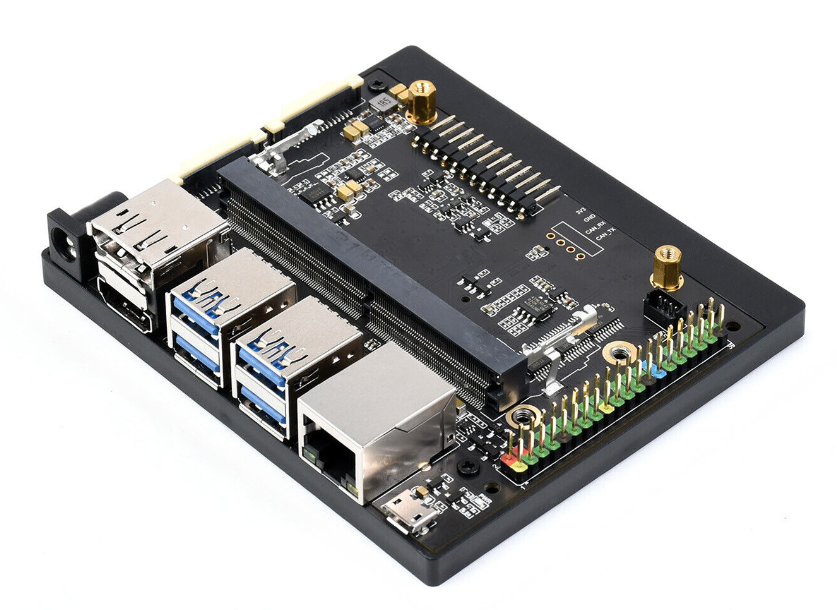
\includegraphics[scale=0.2]{Capitulo3/figs/3 22.png} 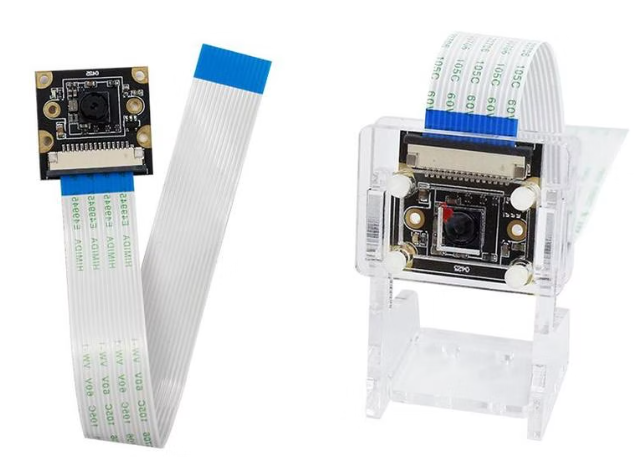
\includegraphics[scale=0.2]{Capitulo3/figs/3 23.png} 
    \caption{Carga útil:Tajera Jetson Nano y cámara IA NVIDIA}
    \label{Carga útil:Tajera Jetson Nano y cámara IA NVIDIA}
\end{figure}

%%%%%%%%%%%%%%%%%%%%%
El \textbf{peso de aviónica} de EHEKATL BWB es de $0.225kg$. está integrado por el kit estándar del controlador de vuelo Pixhawk.

\textit{Auto-piloto} \\
Pixhawk es un hardware de control de vuelo de código abierto. Corre con los ambientes de PX4 y Ardupilot.
\textit{Especificaciones}: 
32 bit ARM Cortex M4 Processor ejecutando NuttX RTOS, 14 salidas PWM/Servo (8 con tolerancias a fallos y anulación manual, 6 auxiliares compatibles con alta potencia), Entradas de alimentación redundantes y conmutación automática, Indicador de audio piezo de alta potencia y multitono, Aplicaciones: Navegación y localización, investigación y educación, control y sistemas estabilizados, Frecuencia: 168 Mhz, RAM: 256 KB, Memoria: 2MB Flash, Almacenamiento: SDCard port, Dimensiones: 81.5x50x15.5mm, Peso: 38g, IMU: giroscopio, Acelerómetro y barómetro; Kit estándar: receptores de telemetría, tarjeta 4G TF, botón de seguridad, zumbador, codificador PPM, placa de expansión I2C, 3 líneas, M8N GPS, soporte GPS, módulo de potencia 3DR y amortiguador. 

\begin{figure}[!h]
    \centering
    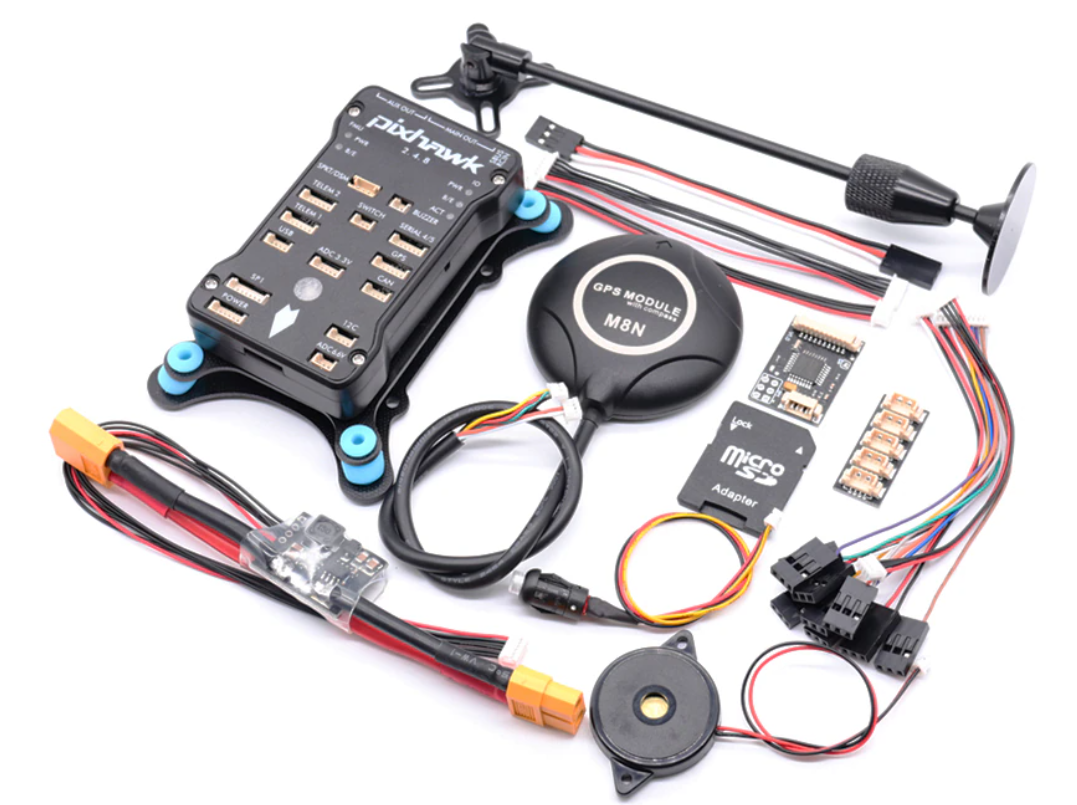
\includegraphics[scale=0.25]{Capitulo3/figs/3 17.png} 
    \caption{Aviónica}
    \label{fig:enter-label}
\end{figure}

%%%%%%%%%%%%%%%%%%%%%%%%%%%%%%%%%%%%%%%
El \textbf{peso del sistema de energía} puede analizarse de diferente manera: si consume  combustible la razón de consumo de combustible específica debe considerarse. Para EHEKATL BWB vamos a considerar baterías eléctricas con le objetivo de no emitir gases de combustión. Con la implementación de baterías también se obtiene obtiene simpleza en el mantenimiento. Su peso es de $0.359kg$ cada pieza, siendo un total de $0.718kg$ de las dos baterías.

\textit{Batería} \\
Se seleccionó una batería Zippy con las siguientes especificaciones: Capacidad: 3300mAh, 4S1P/4/celulares 14.8V, Descarga 40C, 359g (considerando todos los componentes), Dimensiones 139x45x30mm, Balance de enchufe JST-XH y Enchufe de descarga: XT60.

\begin{figure}[!h]
    \centering
    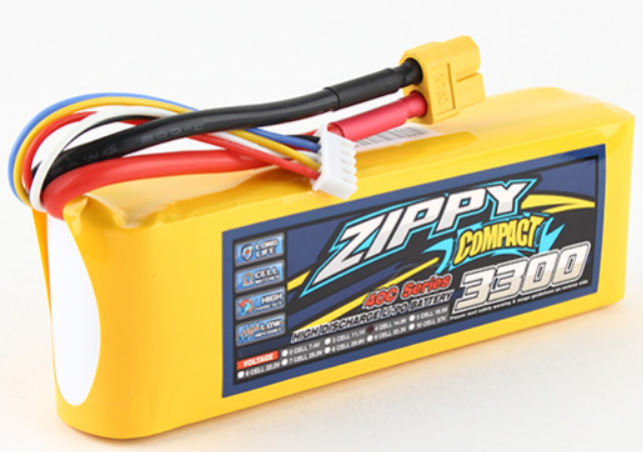
\includegraphics[scale=0.39]{Capitulo3/figs/3 15.png} 
    \caption{Energía}
    \label{Energía}
\end{figure}

El cálculo de la salida de potencia $B_p$ de las baterías refiere a la cantidad de energía eléctrica que la batería puede proveer a una carga en un periodo de tiempo determinado. 
\begin{equation}
\label{battery output power}
    B_p = n I V
\end{equation}
Dónde $n$ es el número de baterías, $I$ la corriente eléctrica y $V$ el voltaje. 
De acuerdo con la batería Zippy seleccionada tenemos las siguientes características:
\begin{itemize}
    \item capacidad de carga: 3300 mAh
    \item voltaje: 22.2 V
    \item tiempo de consumo: 1 hora
    \item no. de baterías: 2
\end{itemize}
Substituyendo en \ref{battery output power} tenemos que: 

\begin{gather}
     B_p = (2) (3300/1000) (22.2) \\
     B_p = 146.52 Wh
\end{gather}
Conectando las baterías en paralelo obtenemos una potencia de salida de $146.52 Wh$.

La densidad energética de la batería refiere a la cantidad de energía que puede ser almacenada en una batería por unidad de volumen. 
\begin{equation}
    E_D = B_p E_c / m_b n
\end{equation}
dónde $E_c$ es el tiempo de consumo de energía en horas  y  $m_b$ la masa de la batería. 
 De acuerdo con nuestras dos baterías Zippy tenemos que:
 \begin{gather}
    E_D = (146.52) (1) / (0.36) (2) \\
    E_D = 203.50 Wh/kg
\end{gather}

Entonces  se establece una densidad energética del sistema de energía de $203.50 Wh/kg$.

Para la fracción del peso del sistema de energía respecto al peso de despegue vamos a establecer la estimación de los siguientes parámetros: $C_L / C_D = 15.38$, una eficiencia de los motores ductofan o hélice de  $\eta  = 0.81$ y un rango de operación de  $R= 12,060 m$.

\begin{gather}
    \frac{W_B}{W_{TO}} = 1.05 (\frac{g}{E_D \eta 3600} \frac{R}{C_L/C_D}) \\
    \frac{W_B}{W_{TO}} = 0.0136
\end{gather}

\medskip

El \textbf{peso vacío} está integrado por:
\begin{itemize}
    \item aero-estructura
    \item motores
    \item tren de aterrizaje
    \item sistemas
\end{itemize}

Hasta el momento no tenemos dimensiones en la geometría de EHEKATL BWB, por lo tanto, la fracción correspondiente del peso vacío respecto al peso máximo de despegue no se puede calcular analíticamente. 

Basándonos en datos históricos con el fin aplicar una regresión lineal la fracción del peso al vacío se puede expresar la siguiente relación. 
\begin{equation}
\label{peso vacío equation}
    \frac{W_E}{W_{TO}}= a W_{TO} + b
\end{equation}


\begin{table}[!h]
    \centering
    \begin{tabular}{|c|c|}
    \hline
    a & b \\
    \hline
     $-4.6^-5$& $0.68$  \\
    \hline
    \end{tabular}
    \caption{Coeficientes de pendiente e intercepto para la estimación del peso vacío de aeronaves de pequeña escala construidas en taller o casa \cite{Sadraey2013}}
    \label{coeficientes del peso al vacío}
\end{table}

Substituyendo los valores de \ref{coeficientes del peso al vacío} en \ref{peso vacío equation} tenemos: 

\begin{equation}
\label{peso vacío equation}
    \frac{W_E}{W_{TO}}= -4.6^-5 W_{TO} + 0.68
\end{equation}

El \textbf{peso máximo de despegue} lo podemos describir de manera intuitiva como la sumatoria de los pesos de la carga útil $W_{PL}$, el sistema de control de vuelo o aviónica $W_{A}$, el sistema de energía $W_{B}$ y el peso al vacío $W_{E}$:

\begin{equation}
    W_{TO} = W_{PL} + W_{A} + W_{B} + W_{E}
\end{equation}

La ecuación anterior también puede ser expresada considerando los factores de peso vacío ($W_E/W_{TO}$) y sistema de energía ($W_B/W_{TO}$). Se suele utilizar el sufijo \textit{B} para baterías y \textit{F} para combustible en el caso de la fracción del sistema de energía. 
\begin{equation}
\label{peso de despegue fracc}
    W_{TO} = \frac{W_{PL}+W_{A}}{1-\frac{W_B}{W_{TO}}-\frac{W_E}{W_{TO}}}
\end{equation}

Actualizamos el valor de $b$ en $0.78$ para obtener un mayor peso de despegue y nos permita cierta holgura en decisiones posteriores de estructura y manufactura. Substituyendo \ref{peso vacío equation} en \ref{peso de despegue fracc} e igualando a cero obtenemos una ecuación cuadrática respecto al peso de despegue o peso máximo de despegue:

\begin{equation}
\label{ecuación cuadrática de peso la vacío}
    -4.6^-5 W_{TO}^2 + (1-0.78-\frac{W_B}{W_{TO}})W_{TO} - (W_{PL}+W_{A})=0
\end{equation}

 
Solucionando la ecuación \ref{ecuación cuadrática de peso la vacío} y tomando el raíz positiva calculamos obtenemos el siguiente peso máximo de despegue:

\begin{table}[h]
    \centering
    \begin{tabular}{|c|c|c|}
    \hline
     \multicolumn{3}{|c|}{Peso máximo de despegue $W_{TO}$} \\
     \hline
    $6.31 kg$ & $61.86 N$ & $13.91 lb$ \\
     \hline
    \end{tabular}
    \caption{Peso máximo de despegue}
    \label{peso maximo de despegue}
\end{table}

De acuerdo con los cuatro pesos que integran el peso de despegue para EHEKATL BWB se muestra la tabla 
%%%%%%%%%%%%%%%%%%%%%%%%%%%%%%%%%%%%%%%%%%%%%%%%%%%%%%%%%%%%%%%%%%%%%%%%%%%%%%%%%%%%%%%%%%%%
\begin{table}[!h]
    \centering
    \begin{tabular}{|c|c|c|c|c|}
    \hline
    \multicolumn{5}{|c|}{Desglose de pesos de EHEKATL BWB}\\
    \hline
     \textbf{$W_{TO}$} & \textbf{$6.31 kg$} & \textbf{$61.86 N$} & \textbf{$13.91 lb$} & $100 \% $  \\
     \hline
      $W_{PL}$ & \textit{$0.30 kg$} & \textit{$2.94  N$} & \textit{$0.66 lb$} & $ 4.75 \% $\\
      $W_{A}$  & \textit{$1.00 kg$} & \textit{$9.81  N$} & \textit{$2.20  lb$} &  $ 15.84 \% $  \\
      $W_{B}$  & \textit{$0.72 kg$} & \textit{$7.06  N$} & \textit{$01.59 lb$} &  $ 11.41 \% $ \\
      $W_{E}$  & \textit{$4.29 kg$} & \textit{$42.05  N$} & \textit{$9.45 lb$} &  $ 67.98 \% $ \\
    \hline
    \end{tabular}
    \caption{Desglose y porcentaje de pesos que integran el peso de despegue de EHEKATL BWB}
    \label{desglose y porcentaje de pesos}
\end{table}


El peso de vacío se considero en base a los coeficientes seleccionados y solamente  se usa como una aproximación en esta etapa el proyecto.

\bigskip
%%%%%%%%%%%%%%%%%%%%%%%%%%%%%%%%%%%%%%%%%%%%%%%%%%%%%%%%%%%%%%%%%%%%%%%%
\textbf{Velocidad de entrada en pérdida}\\
La velocidad de pérdida se refiere a al velocidad mínima que debe tener una aeronave antes de perder sustentación y entrar en pérdida. Solamente helicópteros y vehículos con capacidad de despegue vertical (\textit{VTOL por sus siglas en inglés})  son capaces de volar sin una velocidad hacia adelante. 
La velocidad de entrada en pérdida depende del tipo de aeronave, su peso y el ángulo de ataque. 

En la ecuación de fuerza de levantamiento, así como la velocidad de la aeronave disminuye el coeficiente de levantamiento debe incrementar, hasta encontrar la velocidad de pérdida. 
Una aeronave debe poder estar en equilibrio longitudinal en la condición de vuelo crucero y dentro del rango de velocidades que va desde la velocidad de pérdida hasta la velocidad máxima. 

Durante el vuelo crucero a una velocidad de entrada en pérdida, el peso de la aeronave $W_{TO}$ debe ser balanceado con la fuerza de levantamiento $L$. 
\begin{equation}
\label{sustentación}
    L = W_{TO} = \frac{1}{2} \rho V_s^2 S C_{L_{max}}
\end{equation}
Trabajando el área de referencia en ambos lados de la ecuación \ref{sustentación} obtenemos el primer parámetro para la selección del punto de diseño con \textit{Matching Plot}. 
\begin{gather}
\label{velocidad de perdida}
    (\frac{W}{S})_{V_{s}} = \frac{1}{2} \rho V_s^2  C_{L_{max}} \\
    (\frac{W}{S})_{V_{s}} = \frac{1}{2} (0.9664) (19)^2 (0.48) \\
    (\frac{W}{S})_{V_{s}} = 83.74 N/m^2
\end{gather}
Este resultado es general, tanto para motores jet como motores de propelas. 
%
El resultado en el sistema internacional de \textbf{$83.74 N/m^2$} es equivalente a \textbf{$1.75 lbf/ft^2$}. 
\begin{figure}[!h]
\centering
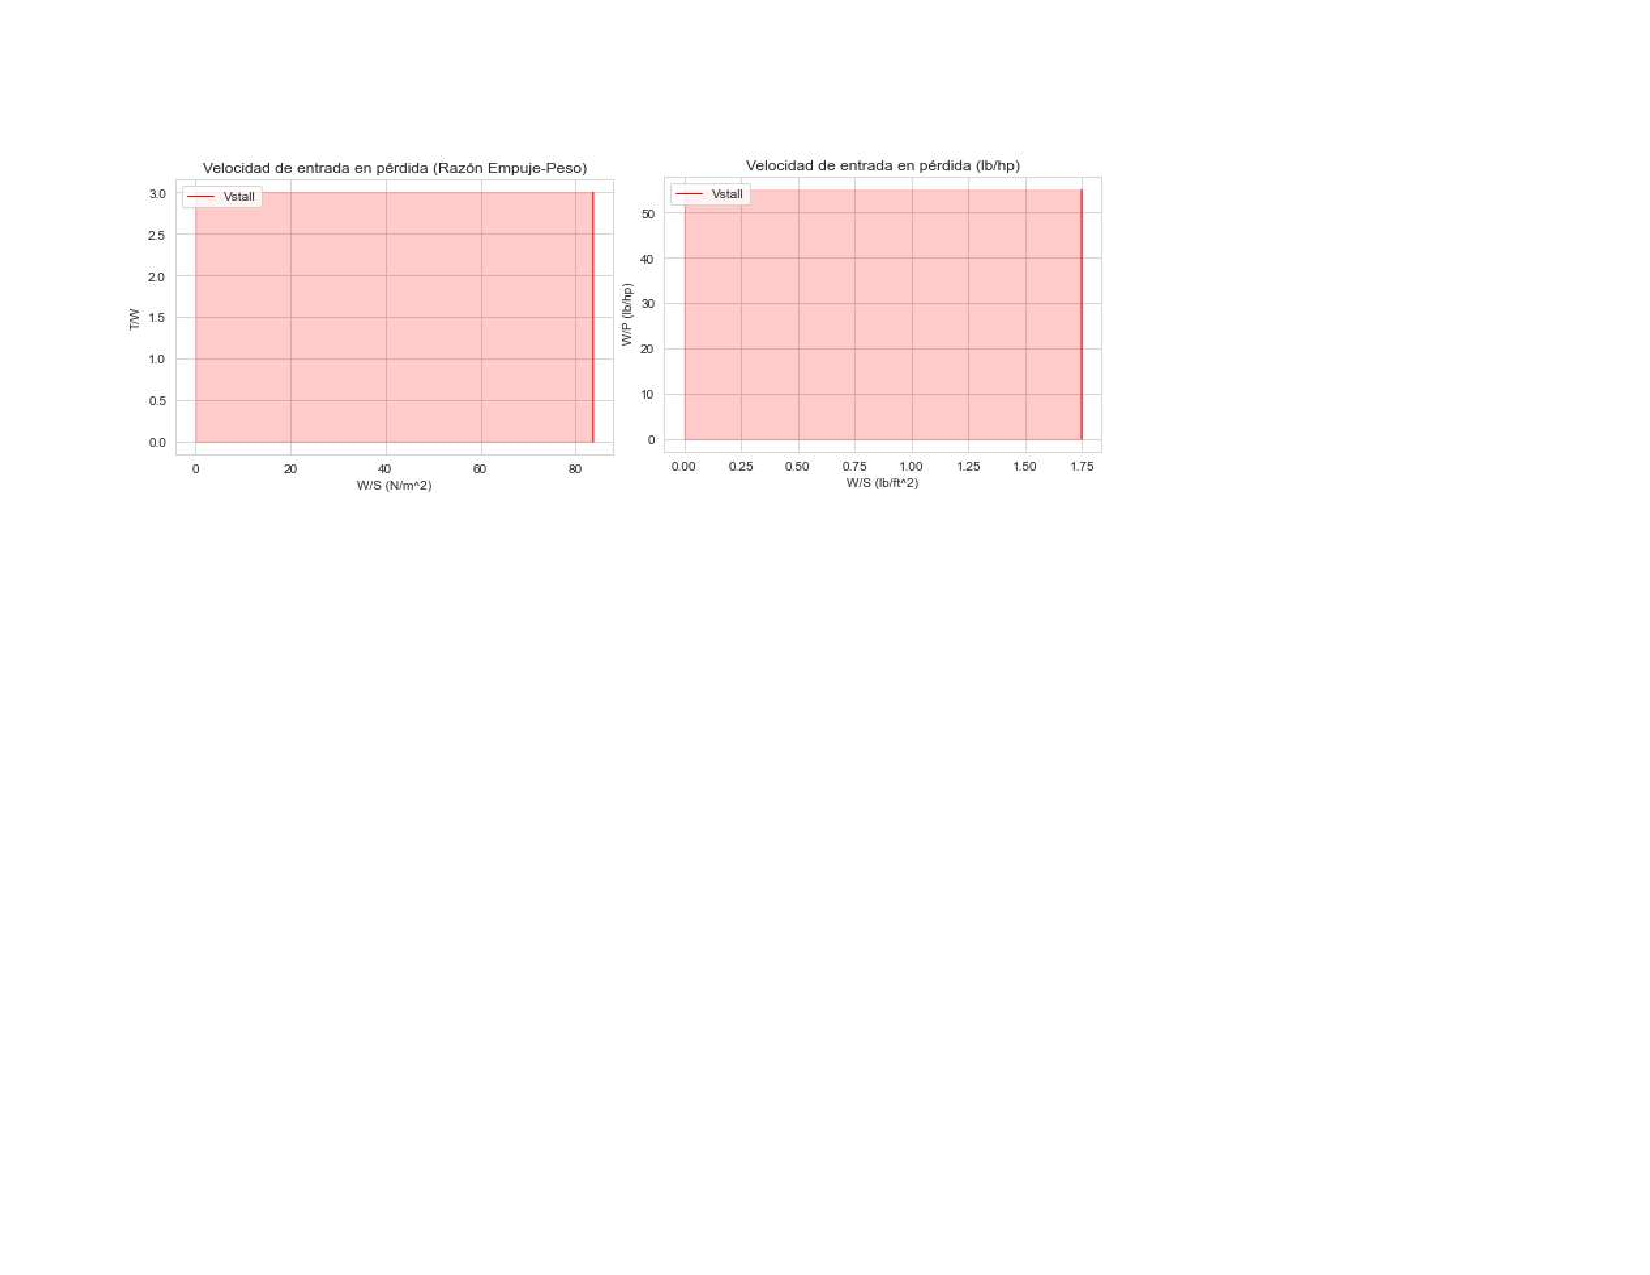
\includegraphics[scale=0.82]{Capitulo3/figs/Vstall_cropped.pdf}
\caption{Velocidad de entrada en pérdida}
\label{Vstall}
\end{figure}

\bigskip
%%%%%%%%%%%%%%%%%%%%%%%%%%%%%%%%%%%%%%%%%%%%%%%%%%%%%%%%%%%%%%%%%%%%%%%%
\textbf{Velocidad máxima}

La velocidad máxima es otro factor decisivo en la esquematización de \textit{Matching Plot}. 
Para motores a reacción consideremos que la aeronave vuela a su velocidad máxima constante a una altitud específica. La aeronave está en equilibrio longitudinal, por tanto, el máximo poder de los motores $T_{max}$ será igual al máximo arrastre $D_{max}$ y el peso $W_{TO}$ de la aeronave será igual al levantamiento $L$:
\begin{gather}
    T_{max} = D_{max} \\
    W = L
\end{gather}

Dónde el levantamiento y el arrastre se definen como:

\begin{gather}
    D = \frac{1}{2} \rho V_{max}^2 S C_D \\
    L = \frac{1}{2} \rho V_{max}^2 S C_L
\end{gather}

Es importante mencionar que el empuje de los motores decrece conforme la altitud incrementa. 
El empuje varia con la velocidad del aire y la altitud. 

\begin{equation}
    T_{alt} = T_{SL} \frac{\rho}{\rho_0} = T_{SL} \sigma
\end{equation}

El sufijo $SL$ alude al nivel del mar. La razón de la densidad es la densidad en la altitud de vuelo respecto la densidad al nivel del mar.

Si dijimos que el empuje máximo es igual al arrastre máximo , entonces podemos definir la siguiente ecuación. 

\begin{equation}
\label{empuje nivel del mar}
    T_{SL} \sigma = \frac{1}{2} V_{max}^2 S C_D
\end{equation}

El \textbf{coeficiente de arrastre} se divide en dos tipos principalmente: \textbf{arrastre de cero-levantamiento $C_{D_0}$} y \textbf{arrastre inducido por levantamiento $C_{D_i}$}:

\begin{equation}
    C_D = C_{D_0} + C_{D_i} = C_{D_0} +  K C_{L}^2 
\end{equation}

dónde $K$ es el factor de arrastre inducido definido como:

\begin{equation}
    K = \frac{1}{\pi e AR}
\end{equation}

dónde $e$ es el factor de eficiencia en evergadura de Oswald, que normalmente va de entre $0.7$ y $0.95$. 


El coeficiente de sustentación puede expresarse en función del peso. 

\begin{equation}
\label{levantamiento peso}
    C_{L} = \frac{2W}{\rho V_{max}^2 S}
\end{equation}

El \textit{coeficiente de arrastre cero-levantamiento $C_{D0}$} es otro parámetro fundamental en los cálculos de \textit{matching plot}. 
También se le conoce como coeficiente de arrastre parásito. Es una medida de arrastre generado por un objeto que se mueve a través de un fluido. Este tipo de arrastre se le conoce de igual forma como de fricción de piel o arratre viscoso. Es generado por la geometría, dimensión y textura de la superficie de la aeronave; y no por la producción de sustentación. 
El arrastre inducido, también conocido como factor de arrastre inducido por sustentación, es una medida de la producción de arrastre respecto a la generación de levantamiento. 

\begin{table}[h]
    \centering
    \resizebox{14cm}{!} {
    \begin{tabular}{|c|c|c|}
    \hline
         & \textbf{Arrastre Parásito } & \textbf{Arrastre Inducido}\\
         \hline
      Peso   &  No influye & Incrementa con el aumento del peso\\
      Velocidad & Incrementa con el aumento de velocidad & Disminuye con el aumento de velocidad\\
      Altitud & Decrece conforme la altitud  & Incrementa conforme la altitud\\
      Ángulo de ataque & No afecta & Aumenta con el aumento del ángulo de ataque\\
      \hline
    \end{tabular}
    }
    \caption{Arrastre parásito vs Arrastre inducido}
    \label{Arrastre parásito vs Arrastre inducido}
\end{table}

La ecuación para calcular el coeficiente de arrastre cero-levantamiento en motores a reacción es la siguiente:

\begin{equation}
    C_{D_0} = \frac{2 T_{SL_{max}} - \frac{4 K W^2}{\rho \omega V_{max}^2 S}} {{\rho_{0} V_{max}^2 S}}\\
\end{equation}

La ecuación para calcular el coeficiente de arrastre cero-levantamiento con motores de hélices es la siguiente:

\begin{equation}
    C_{D_0} = \frac{2 \frac{P_{SL_{max}} \eta_{P}}{V_{max}}  - \frac{4 K W^2}{\rho \omega V_{max}^2 S}} {\rho_{0} V_{max}^2 S} \\
\end{equation}

\medskip

A través del álgebra desarrollamos la ecuación \ref{levantamiento peso} en \ref{empuje nivel del mar}, y despejando el término $\frac{T}{W}$ obtenemos:

\begin{equation}
    (\frac{T_{SL}}{W})_{V_{max}} = \rho_0 V_{max}^2 C_{D_{0}} \frac{1}{2 \frac{W}{S}} + \frac{2K}{\rho \sigma V_{max}^2} \frac{W}{S}
\end{equation}

La razón de la carga de empuje $(\frac{T}{W})$ es una función no lineal respecto a la carga alar $(\frac{W}{S})$. En medida en que se aumenta la velocidad máxima también incrementa la razón de empuje-peso. 
La velocidad máxima suele ser entre un $20-30 \%$ por encima de la velocidad crucero.
La región aceptable para el punto de diseño con motores a reacción se muestra sombreada por encima de la curva en azul.

Cuando consideramos un sistema de propulsión con hélices o propelas, el máximo poder disponible en los motores $P_{max}$ debe ser igual a la máxima potencia requerida $P_{req}$, que es el empuje multiplicado por la máxima velocidad:

\begin{equation}
    P_{req} = \eta_{P} P_{max} = T V_{max}
\end{equation}

dónde el empuje $T$ debe ser igual al arrastre $D$. Entonces tenemos:

\begin{equation}
    \eta_{P} P_{SL} \sigma = \frac{1}{2} \rho V_{max}^2 S C_{D} =  \frac{1}{2} \rho V_{max}^3 S C_{D}
\end{equation}

Desarrollando la ecuación anterior con las mismas consideraciones que hicimos en el empuje de motores jet, obtenemos:

\begin{equation}
    (\frac{W}{P_{SL}})_{V_{max}} = \frac{\eta_{P}}{\frac{1}{2} \rho_{0} V_{max}^3 C_{D_{0}} \frac{1}{(\frac{W}{S})} + \frac{2K}{\rho \sigma V_{max}} (\frac{W}{S})}   
\end{equation}

En $\frac{W}{P}$ cuando incrementa el valor de la velocidad máxima el poder de carga $\frac{P}{W}$ decrece. Esto es debido a que en el primer término de la ecuación tenemos $V_{max}^3$. La región aceptable es por debajo de la curva, contrario al cálculo en motores Jet, ver figura \ref{Vmax}.

\begin{figure}[!h]
\centering
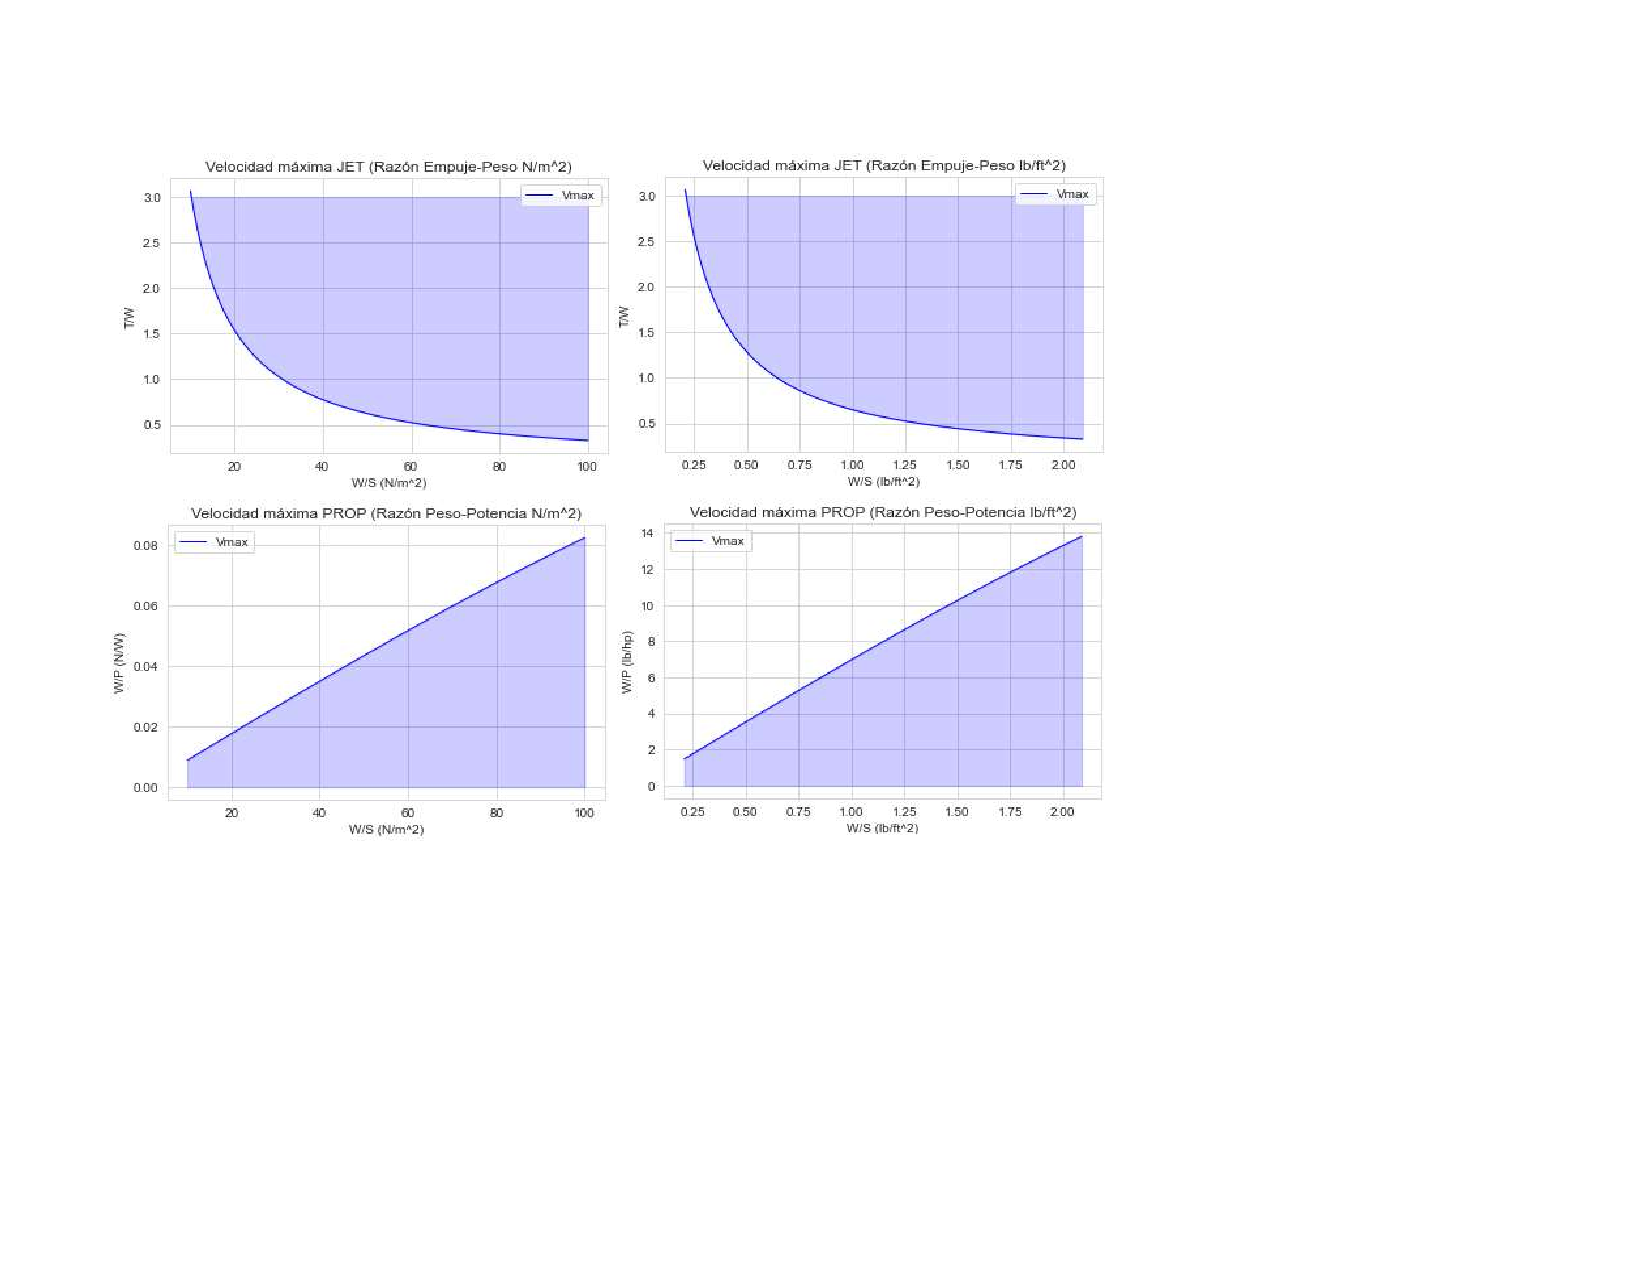
\includegraphics[scale=0.82]{Capitulo3/figs/Vmax_cropped.pdf}
\caption{Velocidad máxima}
\label{Vmax}
\end{figure}


\bigskip
%%%%%%%%%%%%%%%%%%%%%%%%%%%%%%%%%%%%%%%%%%%%%%%%%%%%%%%%%%%%%%%%%%%%%%%%
\textbf{Largo de pista de despegue}\\
Los requerimientos de despegue están asociados con el largo mínimo requerido de la pista de despegue. 

El largo de la pista de despegue está definido como el punto dónde empiezan a acelerar los motores hasta dónde el vehículo aéreo genera cierta sustentación que le hace rebasar una altura pre-establecida. 
De acuerdo con la estándares de la aviación \cite{Sadraey2013} basados en FAR parte 25, la altura pre-establecida que debe alcanzar el vehículo aéreo al final de la pista es de $35 pies$ o $10.7 m$ para aeronaves de pasajeros. 
Sin embargo, la FAR no establece un requerimiento estricto para el largo de la pista de despegue. 

Para motores Jet o de reacción vamos a utilizar la siguiente ecuación.

\begin{equation}
    (\frac{T}{W})_{S_{TO}} = \frac{\mu - (\mu + \frac{C_{D_G}}{C_{L_R}})[exp(0.6 \rho g C_{D_G} S_{TO} \frac{1}{W/S})]}{1 - exp(0.6 \rho g C_{D_G} S_{TO} \frac{1}{W/S})}
\end{equation}

Dónde $\mu$ es el coeficiente de fricción de la pista de despegue y $C_{D_G}$ se define como:
\begin{equation}
    C_{D_G} = (C_{D_{TO}} - \mu C_{L_{TO}})
\end{equation}
Dónde el sufijo $TO$ hace referencia a los parámetros aerodinámicos en configuración de despegue. 
El parámetro $C_{L_R}$ es el coeficiente de levantamiento durante la rotación y se obtiene:
\begin{equation}
    C_{L_R} = \frac{2 m g }{\rho S V_R^2}
\end{equation}
Dónde $V_R$ es la velocidad de rotación durante el despegue y normalmente es entre $15-30 \%$ mayor que la velocidad de desplome. 
Si el vehículo aéreo utiliza \textit{flaps} para el despegue debe considerarse la suma de la contribución de este efector en el coeficiente de levantamiento. 

En conclusión para motores Jet, en medida en que el largo de la pista de despegue incrementa, el valor de la razón de empuje-peso disminuye. Dado que cualquier valor por encima del largo mínimo establecido $S_{TO}$ no satisface los requerimientos en empuje durante el despegue, la parte por debajo de la curva no es aceptable.   

Para motores de hélice vamos a utilizar la siguiente expresión:
\begin{equation}
    (\frac{W}{P})_{S_{TO}} = \frac{1 - exp(0.6 \rho g C_{D_G} S_{TO} \frac{1}{W/S})}{\mu - (\mu + \frac{C_{D_G}}{C_{L_R}})[exp (0.6 \rho g C_{D_G} S_{TO} \frac{1}{W/S})]} \frac{\eta_{P}}{V_{TO}}
\end{equation}
 
La eficiencia para hélices fijas en el momento de cabeceo tienen una eficiencia de $0.5$ mientras que las hélices con cabeceo variable tienen una eficiencia del $0.6$.
En medida en que se incrementa el largo de la pista de despegue, el valor de la carga de potencia se incrementa. La región por encima de la curva no es aceptable. 

\begin{figure}[!h]
\centering
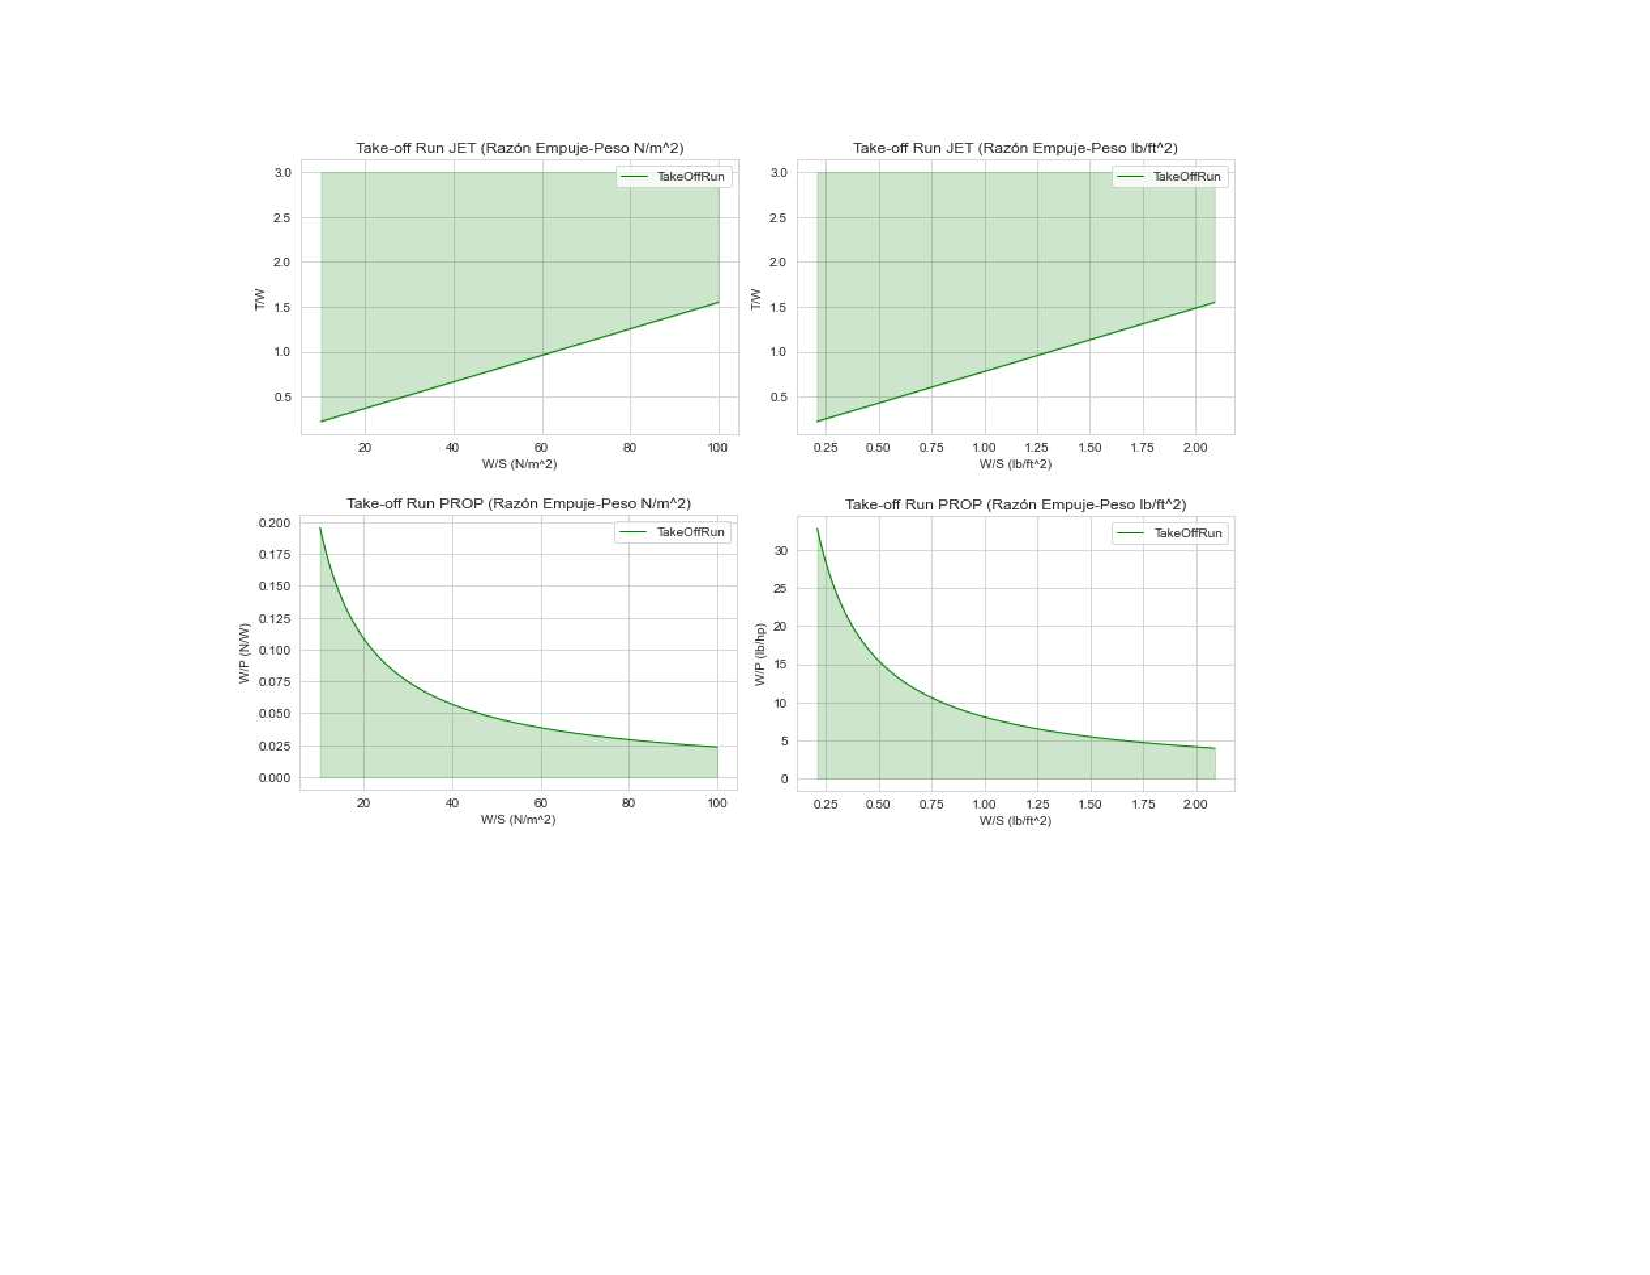
\includegraphics[scale=0.79]{Capitulo3/figs/takeoff run_cropped.pdf}
\caption{Carrera de pista de despegue}
\label{Vtakeoff}
\end{figure}

\bigskip
%%%%%%%%%%%%%%%%%%%%%%%%%%%%%%%%%%%%%%%%%%%%%%%%%%%%%%%%%%%%%%%%%%%%%%%%
\textbf{Régimen  de ascenso}\\
Cada tipo de aeronave debe cumplir con un régimen de ascenso.
La razón de ascenso se define como la velocidad en el eje vertical.
Por tanto, \textit{ROC,por sus siglas en inglés} define que tan rápido el vehículo aéreo gana altitud. 

El ROC para motores a reacción se define como la razón entre el exceso de poder y el peso de la aeronave:
\begin{equation}
    ROC = \frac{P_{avl} - P_{req}}{W} = \frac{(TV - DV)}{W}
\end{equation}
Para maximizar ROC debemos maximizar el empuje de los motores y la polar o razón de levantamiento-arrastre. Entonces podemos reescribir la ecuación anterior en:
\begin{equation}
    ROC = V[\frac{T}{W} - \frac{D}{W}] =  V[\frac{T}{W} - \frac{D}{L}] = V[\frac{T}{W} - \frac{1}{L/D}]
\end{equation}
Y entonces:
\begin{equation}
    ROC_{max} = V_{ROC_{ma}}[\frac{T_{max}}{W}-\frac{1}{(L/D)_{max}}]
\end{equation}
Considerando la minimización del arrastre para el incremento de polar y manipulando algunos términos para tener una función en base a la carga alar obtenemos:
\begin{equation}
    (\frac{T}{W})_{ROC} = \frac{ROC}{\sqrt{\frac{2}{\rho \sqrt{\frac{C_{D_0}}{K}}}(\frac{W}{S})}} + \frac{1}{(L/D)_{max}}
\end{equation}
Para determinar la región aceptable debemos observar que lado de la curva satisface los requerimientos. 
En medida en que incrementa la razón de ascenso, el valor de la carga de empuje $(T/W)$ también incrementa. 
Cualquier valor de ROC mayor al establecido satisface los requerimientos, por lo que el área sobre la curva es la región aceptable. 

para motores de propelas la ecuación es la siguiente:
\begin{equation}
    (\frac{W}{P})_{ROC} = \frac{1}{\frac{ROC}{\eta_{P}} + \sqrt{\frac{2}{\rho \sqrt{\frac{3 C_{D_0}}{K} (\frac{W}{S})} (\frac{1.155}{(L/D)_{max} \eta_P})}}}
\end{equation}

Para este caso en medida que el valor de ROC aumenta, el valor de la carga de empuje $(W/P)$ disminuye. La región por debajo de la curva es la aceptable, ver figura \ref{ROC}. 

\begin{figure}[!h]
\centering
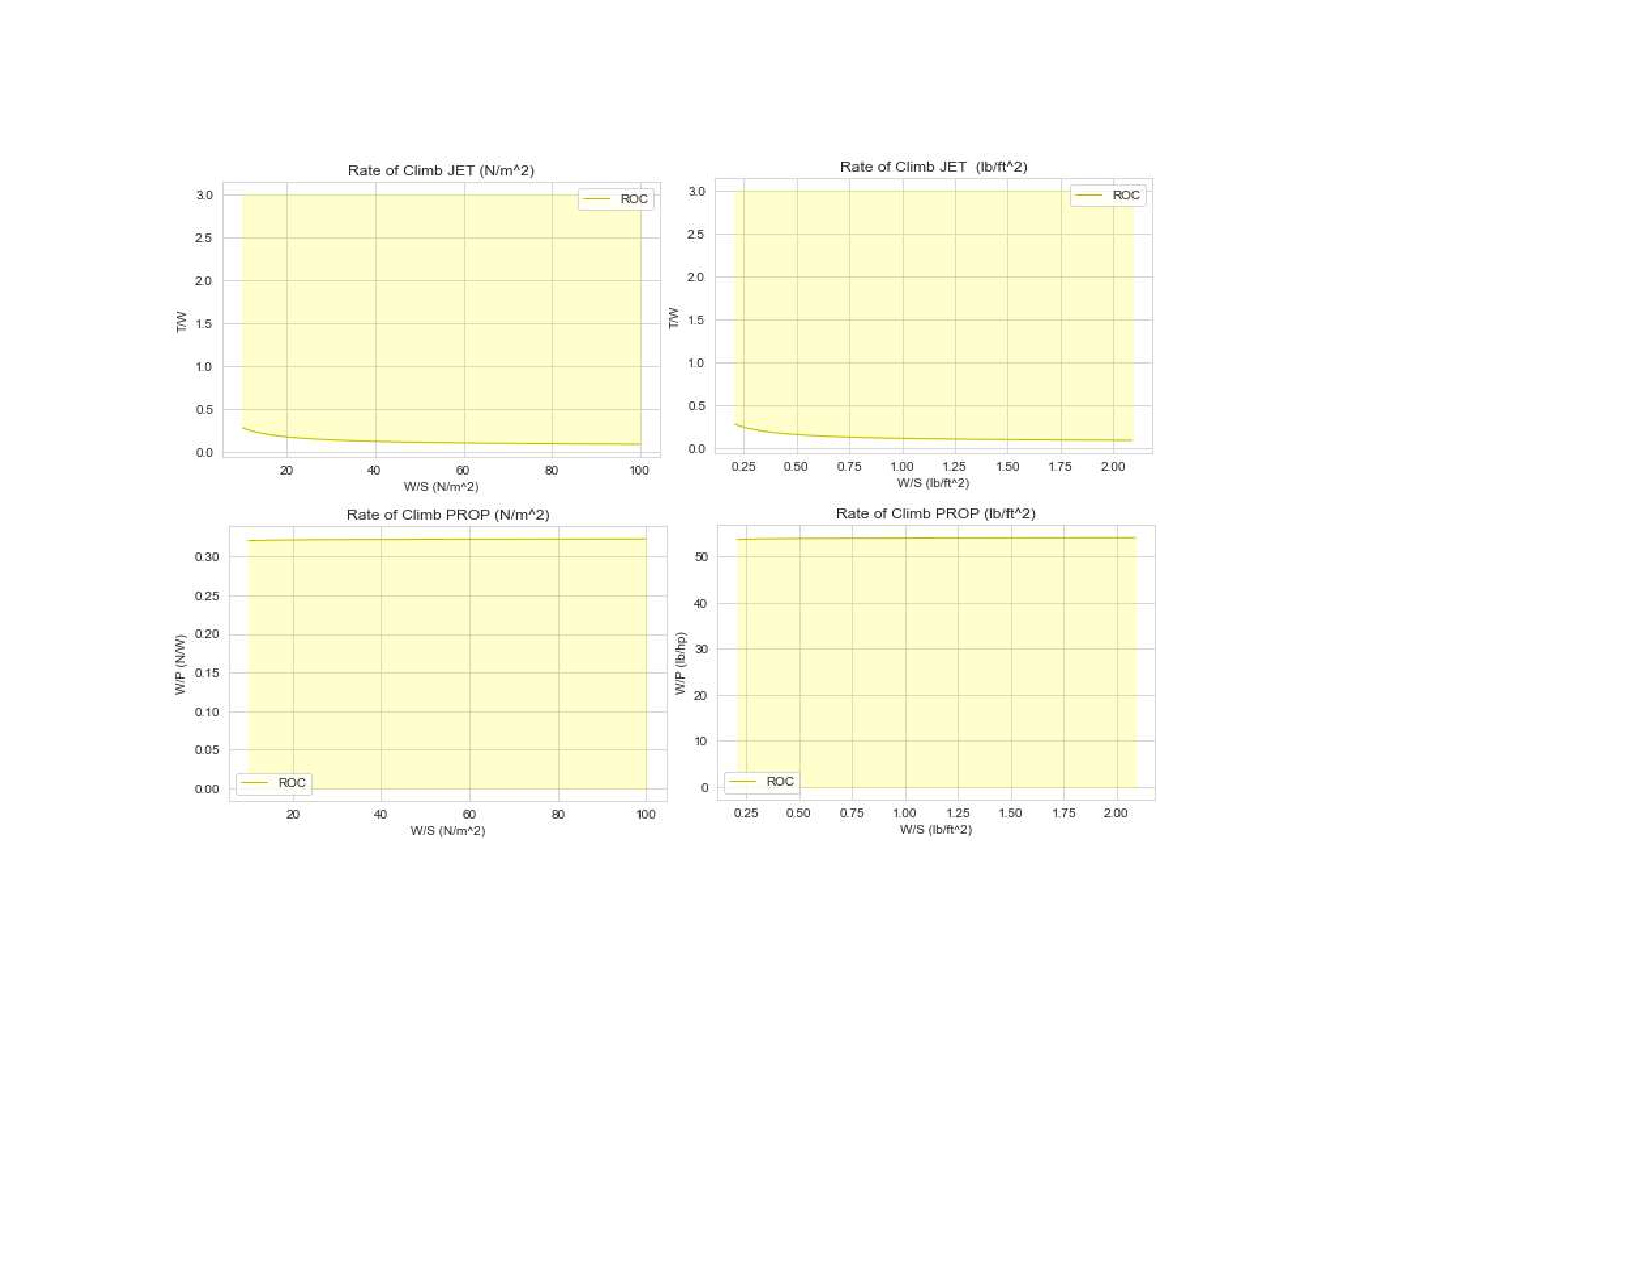
\includegraphics[scale=0.79]{Capitulo3/figs/ROC_cropped.pdf}
\caption{Régimen de ascenso}
\label{ROC}
\end{figure}

\bigskip
%%%%%%%%%%%%%%%%%%%%%%%%%%%%%%%%%%%%%%%%%%%%%%%%%%%%%%%%%%%%%%%%%%%%%%%%
\textbf{Techo de servicio}\\
El \textit{techo} se define como la altitud máxima que el vehículo aéreo puede alcanzar teniendo un seguro vuelo recto y nivelado. 
Otra definición podría ser la máxima altitud para tener un vuelo sostenido de acuerdo con la la máxima propulsión que pueden ofrecer los motores. 
En general, se pueden definir cuatro tipos de techo:
\begin{itemize}
    \item Techo absoluto. Es la altitud máxima que el vehículo aéreo puede mantener un vuelo seguro recto y nivelado. A esta altitud el régimen de ascenso es cero. 
    \item Techo de servicio. Es altitud máxima que el vehículo aéreo puedo alcanzar con un régimen de ascenso de $100 \frac{ft}{min}, o 0.5 \frac{m}{s}$. El Techo de servicio es menor que el techo absoluto. 
    \item Techo crucero. Es la altitud máxima que el vehículo aéreo puede alcanzar con una velocidad de ascenso de $300 \frac{ft}{min}, o 1.5 \frac{m}{s}$.
\end{itemize}
El techo de servicio y crucero están basados en el régimen de ascenso. Para EHEKATL BWB se establecen los siguientes 
\begin{itemize}
    \item[] $ROC_{Absoluto} = 0 m/s$
    \item[] $ROC_{Servicio} = 1.25 m/s$
    \item[] $ROC_{Crucero} = 2.5 m/s$
\end{itemize}
Para motores Jet se plantea la siguiente ecuación:
\begin{equation}
    (\frac{T}{W})_{h_c} = \frac{ROC_c}{\sigma_C  \sqrt{\frac{2}{\rho_c \sqrt{\frac{C_{D_0}}{K} (\frac{W}{S})}}}} + \frac{1}{\sigma_C (L/D)_{max}}
\end{equation}
dónde $h_c$ es el techo requerido máximo para un $ROC_c$ régimen de ascenso específico. 
Cuando el vehículo aéreo está en techo absoluto el ROC es cero, entonces podemos simplificar la ecuación anterior con el siguiente término:
\begin{equation}
    (\frac{T}{W})_{h_{AC}} = \frac{1}{\sigma_{AC} (L/D)_{max}}
\end{equation}
dónde $h_{AC}$ es la altitud del techo absoluto y $\sigma_{AC}$ es la densidad del aire en la relativa de acuerdo con el techo absoluto. 
Para determinar la región aceptable planteamos la siguiente consideración: en medida que decrece el régimen de ascenso el valor de la carga de empuje también decrece. Entonces, cualquier valor de ROC mayor sobre la curva satisface el requerimiento. 
\begin{figure}[!t]
\centering
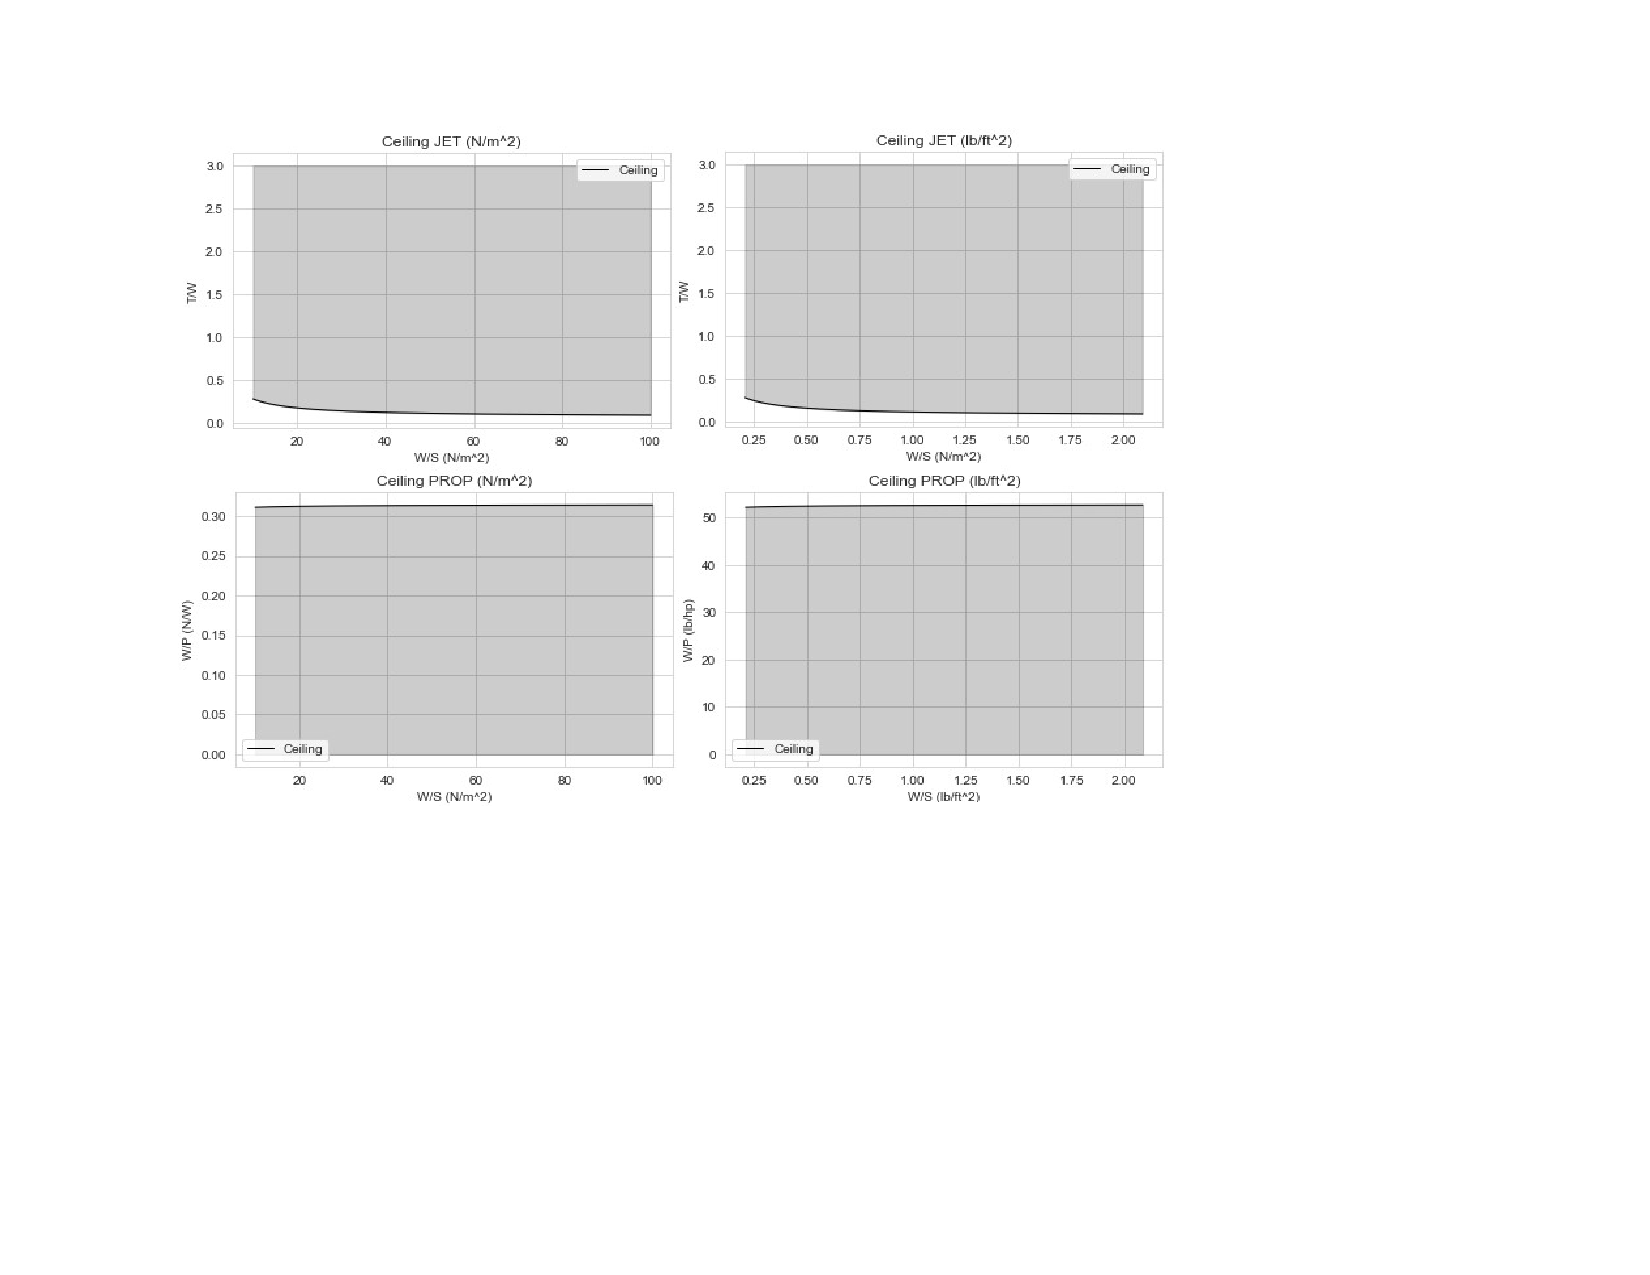
\includegraphics[scale=0.80]{Capitulo3/figs/Ceiling_cropped.pdf}
\caption{Techo de servicio}
\label{Ceiling}
\end{figure}
Para motores de \textbf{hélices o propelas} vamos a emplear la siguiente ecuación.
\begin{equation}
    (\frac{W}{P})_C = \frac{\sigma_C}{\frac{ROC_C}{\eta_P} + \sqrt{\frac{2}{\rho_C \sqrt{\frac{3 C_{D_0}}{K} (\frac{W}{S})} (\frac{1.155}{(L/D)_{max}\eta_P}}}}
\end{equation}
Para el techo absoluto la expresión anterior se puede simplificar de la siguiente manera:
\begin{equation}
    (\frac{W}{P})_{AC} = \frac{\sigma_{AC}}{\sqrt{\frac{2}{\rho_{AC} \sqrt{\frac{3 C_{D_0}}{K} (\frac{W}{S})} (\frac{1.155}{(L/D)_{max} \eta_P})}}}
\end{equation}

\bigskip
%%%%%%%%%%%%%%%%%%%%%%%%%%%%%%%%%%%%%%%%%%%%%%%%%%%%%%%%%
\textbf{Punto de diseño - \textit{Matching Plot}}\\
Ahora que tenemos las curvas de los cinco requerimientos (velocidad de pérdida, velocidad máxima, largo de la pista de despegue, régimen de ascenso y techo de servicio) de acuerdo con la carga de poder o razón de empuje-peso respecto de la carga alar, podemos integrar las cinco funciones en la figura \ref{Punto de Diseño} para seleccionar el punto de diseño. 
%
\begin{table}[!h]
    \caption{Punto de Diseño - Matching Plot}
    \centering
    \begin{tabular}{|c|c|c|c|}
    \hline
    \multicolumn{4}{|c|}{\textbf{Motores Ductofan}}\\
    \hline
    $(\frac{T}{W})_d$ & Razón Empuje-Peso & \multicolumn{2}{|c|}{$0.85$} \\
    \hline
    $(\frac{W}{S}_d$ & Carga Alar &  $45 N/m^2$ & $0.9398 lb/ft^2$\\
    \hline
    \multicolumn{4}{|c|}{\textbf{Motores Hélice}}\\
    \hline
    $(\frac{W}{P})_d$ & Carga de Empuje & $0.03 N/m^2$  & $ lb/ft^2$ \\
    \hline
    $(\frac{W}{S}_d$ & Carga Alar &  $50 N/m^2$ & $1.0442 lb/ft^2$\\
    \hline
    \end{tabular}
    \label{Punto de Diseño Matching Plot}
\end{table}

\begin{figure}[!h]
\centering
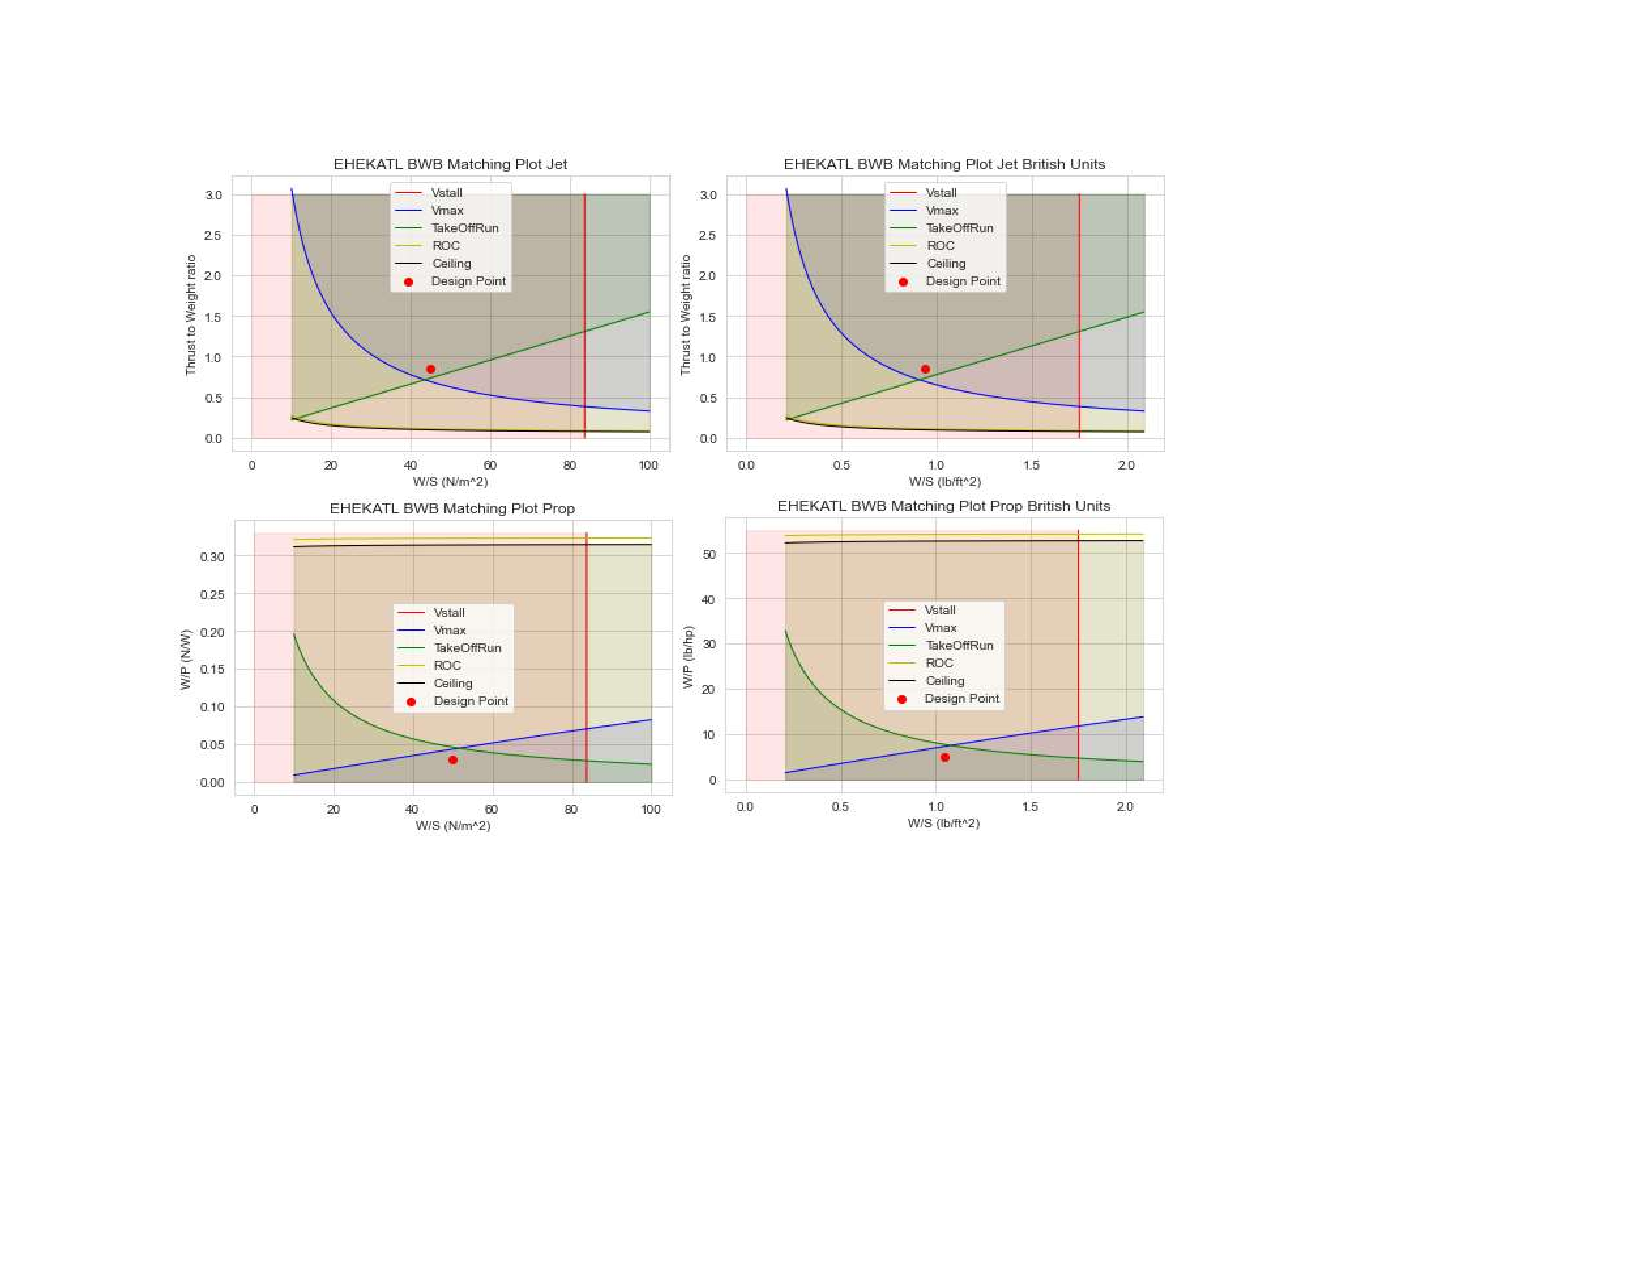
\includegraphics[scale=0.79]{Capitulo3/figs/Matching plot_cropped.pdf}
\caption{Resultados: Punto de Diseño con \textit{Matching Plot}}
\label{Punto de Diseño}
\end{figure}

La región aceptable global, dónde coinciden todos los requerimientos, es la esencia para la selección del punto de diseño en \textit{Matching Plot}. 
%
De acuerdo entonces con la región aceptable mostrada en la figura \ref{Punto de Diseño} el punto de diseño se muestra en la tabla \ref{Punto de Diseño Matching Plot}.

\medskip

Entonces podemos calcular la \textbf{superficie alar} y el \textbf{empuje requerido} de la siguiente manera para los \textbf{motores a reacción}:

\begin{equation}
    S = \frac{W_{TO}}{(\frac{W}{S}_d)} = \frac{62 N}{45 N/m^2} = 1.375 m^2
\end{equation}

\begin{equation}
    T = W_{TO} (\frac{T}{W})_d = 62N (0.85) = 52.60N
\end{equation}

De tal forma que para cumplir los requerimientos de la tabla \ref{Requerimientos de la misión de vuelo} EHEKATL BWB debe tener un área de referencia mínima de $1.375 m^2$ y los motores deben dar un empuje mínimo de $52.60N$ para que nuestro vehículo aéreo pueda despegar de la acera. 

\medskip

Para \textbf{motores hélice} el cálculo de la \textbf{superficie alar} y la \textbf{potencia requerida} es el siguiente:

\begin{equation}
    S = \frac{W_{TO}}{(\frac{W}{S}_d)} = \frac{62 N}{55 N/m^2} = 1.125 m^2
\end{equation}

\begin{equation}
    P = \frac{W_{TO}}{(\frac{W}{P}_d)} = \frac{62 N}{0.033 N/W} = 1,875.06 W
\end{equation}

De tal forma que para cumplir los requerimientos de la tabla \ref{Requerimientos de la misión de vuelo} EHEKATL BWB debe tener un área de referencia mínima de $1.125 m^2$ y los motores deben dar un empuje mínimo de $ 1,875.06 W$ para que nuestro vehículo aéreo pueda despegar. 


En la tabla \ref{Punto de Diseño} se muestran los resultados definitivos de la superificie alar y la potencia/empuje requerido. 

\begin{table}[!h]
    \label{superficie alar y potencia/empuje requeridos para EHEKATL BWB}
    \caption{Superficie Alar y Potencia/Empuje Requeridos}
    \centering
    \begin{tabular}{|c|c|c|c|}
    \hline
    \multicolumn{4}{|c|}{\textbf{Motores Ductofan}} \\
    \hline
      S   &  Superficie Alar & $1.375 m^2$ & $14.80 ft^2$ \\
     T    & Empuje Mínimo Requerido & $52.60N$ & $11.8249 lbf$ \\
     \hline
     \multicolumn{4}{|c|}{\textbf{Motores Hélice}} \\
     \hline
     S   &  Superficie Alar & $1.125 m^2$ & $12.1093875 ft^2$ \\
     P   & Potencia Mínima Requerida & $1,875.06 W$ & $2.5125 hp$ \\
     \hline
    \end{tabular}
\end{table}

En la figura \ref{Punto de Diseño} el esquema de \textit{Matching Plot} tiene dos puntos de optimización dentro de la región aceptable.
%
El primero, en la intersección entre la curva de velocidad de máxima y la pista de despegue. Este punto representa la carga alar y potencia/empuje mínimos requeridos para lograr el despegue y mantener en sustentación el vehículo aéreo. 
%
El segundo, en la intersección de la pista de despegue con la velocidad de entrada en pérdida. Este punto representa la carga alar máxima disponible respecto a la potencia/empuje mínimos requeridos para esa carga.
%
Nuestra selección del punto de diseño fue en base al primer criterio, con carga alar y potencia/empuje mínimos requeridos. 
%
El análisis aerodinámico y de estabilidad presentados en este capítulo contemplan los resultados obtenidos de superficie alar y potencia requerida. 
Se establece un área de superficie alar de $1.4m^2$ para EHEKATL BWB. 
%
Los resultados de potencia requerida se utilizan para las simulaciones de prueba con X-PLANE. 

%%%%%%%%%%%%%%%%

%%%%%%%%%%%%%%%%%%%%%%%%%%%%%%%%%%%%%%%%%%%%
\section{Controlador Proporcional Integral Derivativo}
%%%%%%%%%%%%%%%%%%%%%%%%%%%%%%%%%%%%%%%%%%%%

Sea un controlador Proporcional Integral Derivativo de la forma:
\begin{equation}
    u(t) = K_p e(t) + K_i \int_0^t e(t) dt + k_d \dot e(t), t \geq 0 
\end{equation} 

dónde $K_p , K_i , K_d$ son las matrices de ganancias para la sintonización proporcional, integral y derivativa del error de seguimiento $e(t)$, con $q_d(t)$ como referencia deseada. 
\begin{equation}
    e(t) = q_d(t) - q(t)
\end{equation}
El componente \textbf{proporcional} produce una salida que es proporcional al valor del error actual. 
El componente \textbf{integral} suma el error acumulado en el tiempo para producir una salida que es proporcional al error acumulado. 
La componente de la \textbf{derivada} produce una salida que es proporcional a la razón de cambio del error, \cite{Tewari2013}. 
\begin{figure}[!h]
    \centering
    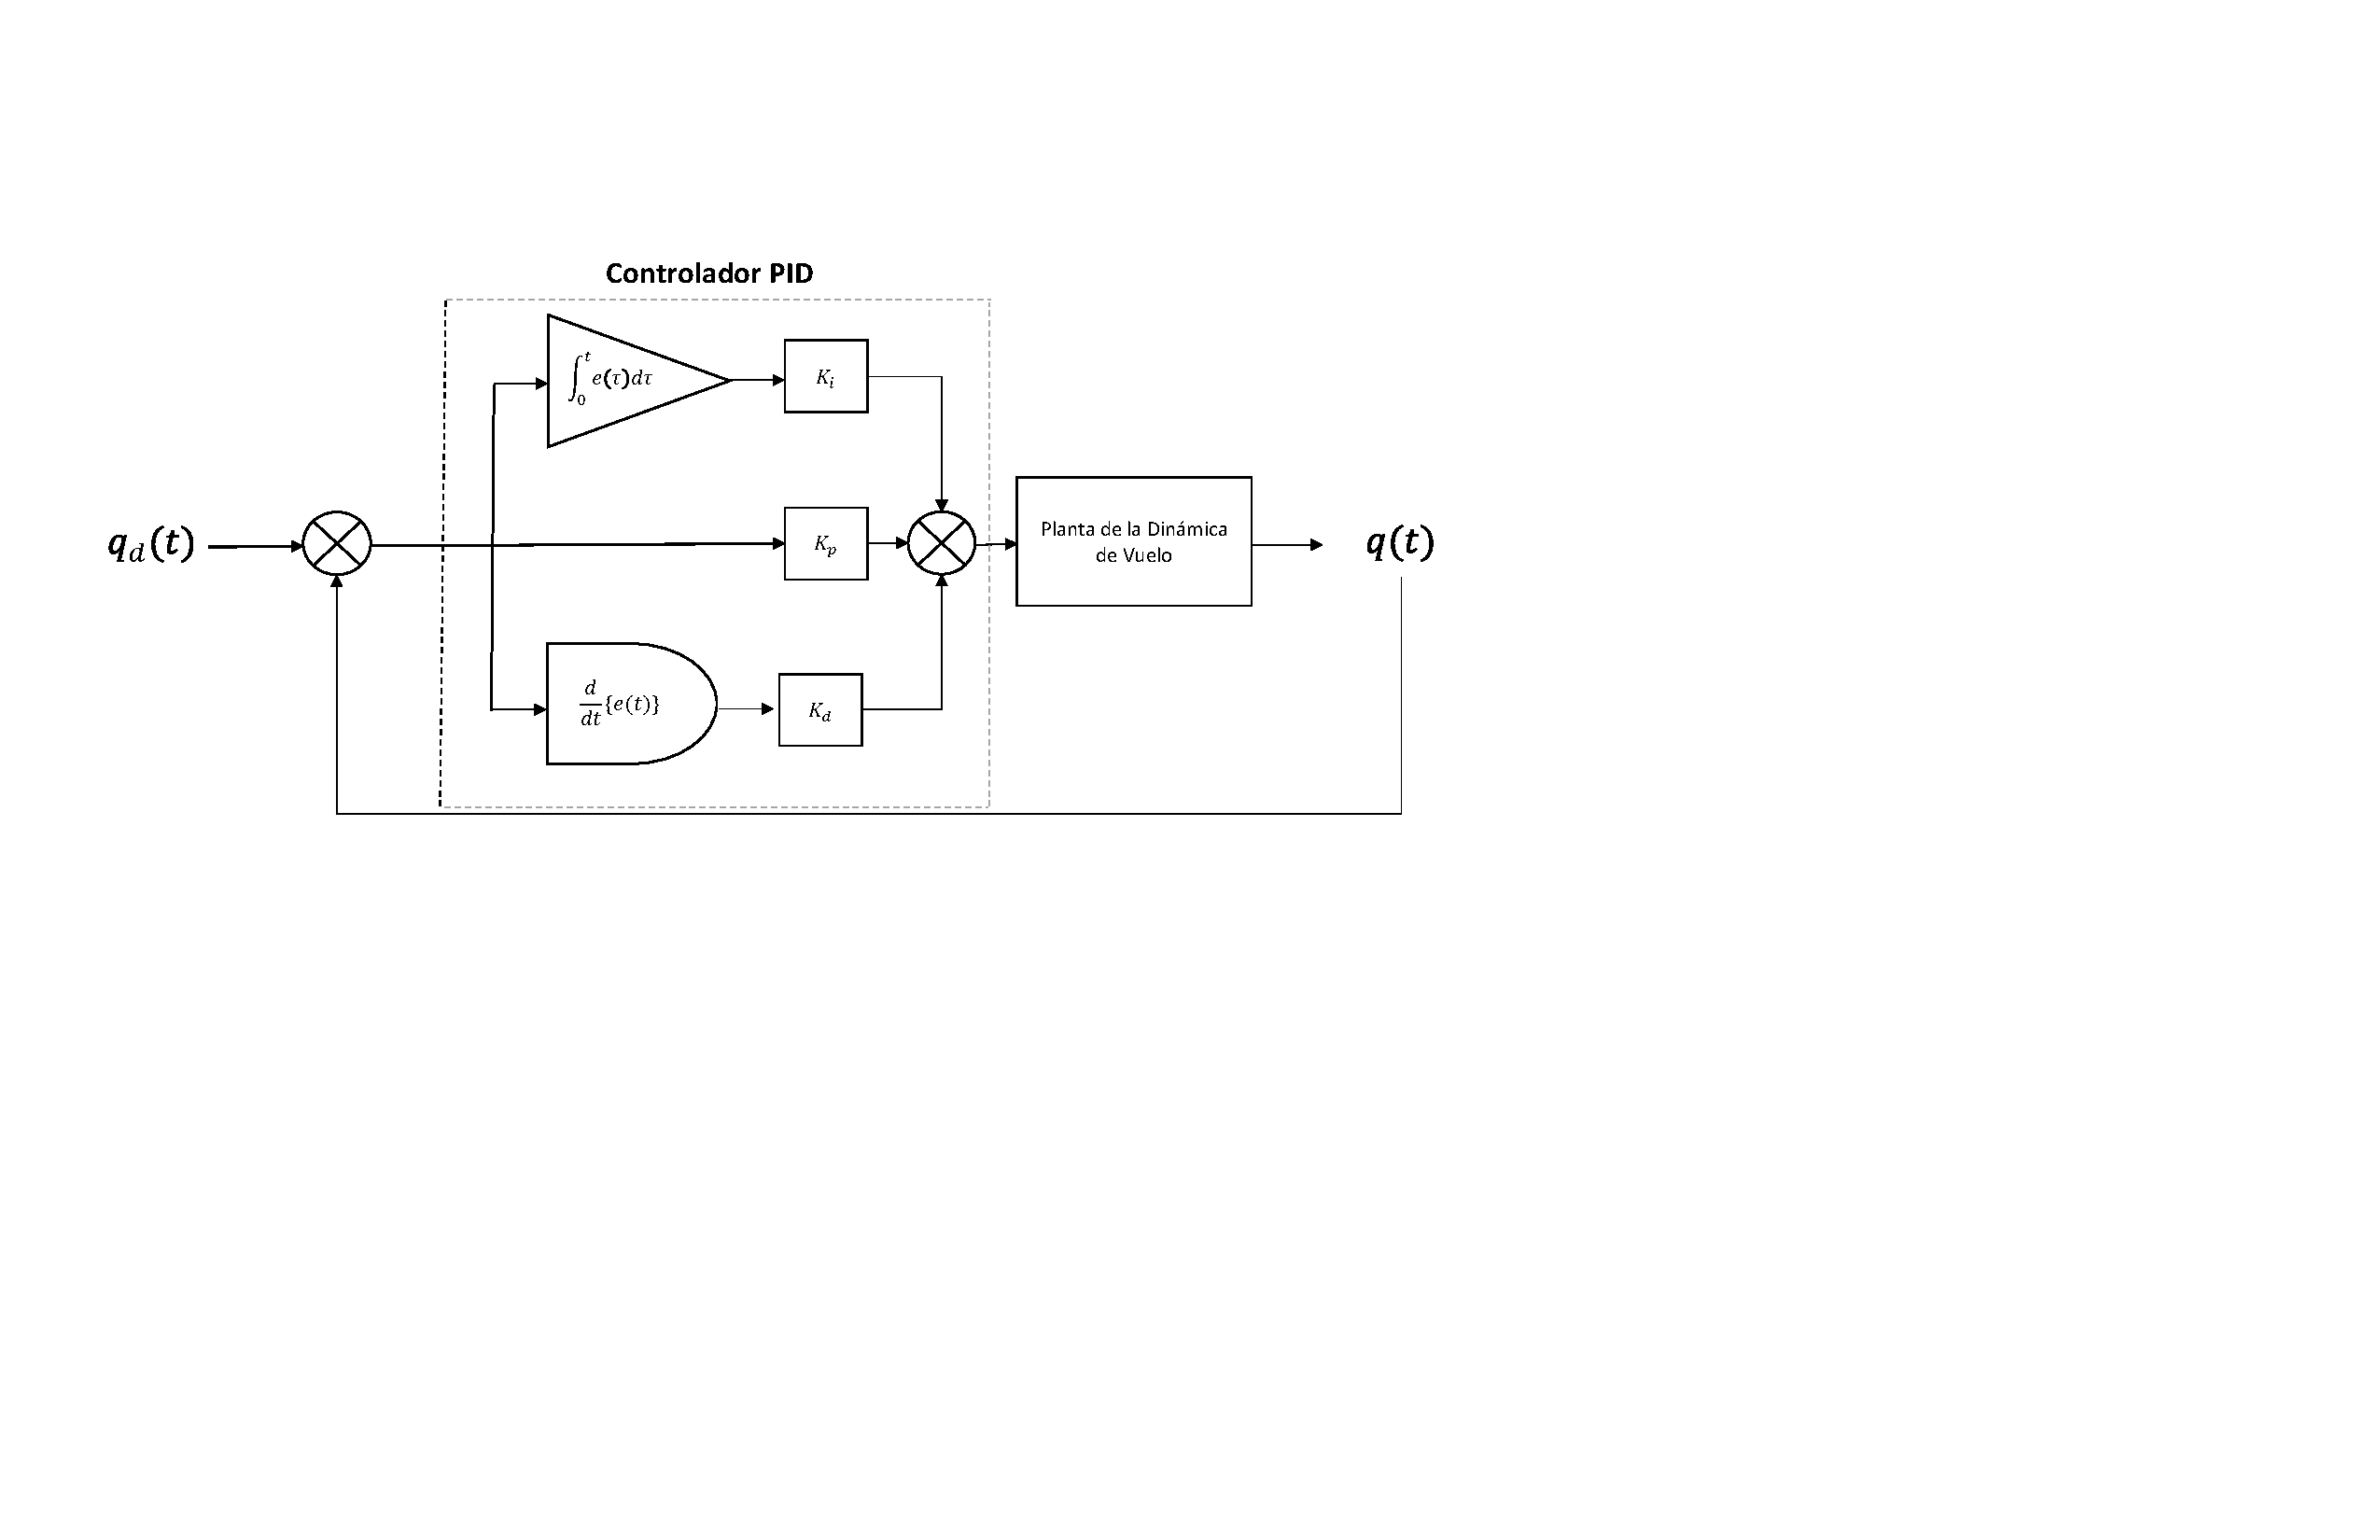
\includegraphics[scale=0.53]{Capitulo3/figs/PID new controller.pdf}
    \caption{Diagrama de bloques del controlador PID}
    \label{fig:PID controller}
\end{figure}


El proceso de determinación de las ganancias se le conoce como \textbf{sintonización}. 
Aunque el control PID fue originalmente desarrollado para sistemas de única variable, su aplicación fue extendida a plantas de variable múltiple. 

El esquema general del controlador PID para EHEKATL BWB se muestra en la figura \ref{fig:PID controller}, \cite{Tewari2013}. 
%
El controlador se diseño como un sistema SISO (\textit{Single-Input, Single-Output} por sus sigla en inglés) de única entrada y única salida. 
Para el control longitudinal se utilizan los elevadores en respuesta al régimen de ascenso \textit{ROC} o la velocidad lineal normal $w$.
Para el control lateral se utilizan los alerones  en relación con la velocidad de alabeo $p$.
Para el control direccional se utilizan los timones en relación con la velocidad de guiñada $r$. 

\bigskip
%%%%%%%%%%
\textbf{Simulación de Control PID para Vuelo Crucero}\\
El vuelo crucero es la fase de la misión de vuelo con mayor duración, y se caracteriza por ser un vuelo dónde la altitud y la velocidad son constantes y la variación en el ángulo de ataque es pequeña, además, es un vuelo a nivel del ala dónde las velocidad angulares de alabeo y guiñada se consideran no significativas y podemos ser negligentes con la dinámica lateral y direccional. 
%
La principal función del controlador de vuelo PID durante el vuelo crucero de EHEKATL BWB es compensar las perturbaciones que pudieran presentarse durante el vuelo  crucero para mantener la actitud de cabeceo y cierto  ángulo de ataque, además, de regir el régimen de ascenso para lograr la altitud deseada. 

La simulación se hará a través de una representación en espacios de estados del modelo lineal longitudinal de EHEKATL BWB visto en \ref{lineal longitudinal cuerpo}-\ref{lineal longitudinal cuerpo 1} considerando un \textbf{sistema continuo invariante en el tiempo}, ver ecuación \ref{longitudinal lineal EHEKATL BWB}.
\begin{equation}
\label{longitudinal lineal EHEKATL BWB}
    \begin{bmatrix}
        \dot u \\
        \dot w \\
        \dot q \\
        \dot \theta
    \end{bmatrix}
    =
    \begin{bmatrix}
    -0.0406476 & 0.651139 & 0 & -9.81 \\
    -1.5108 & -4.21972 & 10.9907 & 0 \\
    -7.04976e-08 & -2.99525 & -4.33042 & 0 \\
    0 & 0 & 1 & 0 \\
    \end{bmatrix}
    \begin{bmatrix}
        u \\
        w \\
        q \\
        \theta
    \end{bmatrix}
    +
    \begin{bmatrix}
    0.4311 \\
    -13.2133 \\
    -27.35 \\
    0\\
    \end{bmatrix}
    \delta_e
\end{equation}

Los parámetros aerodinámicos dimensionales de la ecuación \ref{longitudinal lineal EHEKATL BWB} se obtuvieron a través de un análisis de estabilidad con XFLR5, dónde se consideró una masa $m$ de $6.31kg$ y el análisis de estabilidad arrojo un momento de inercia $I_y$ de $0.8856 kgm^2$ a una velocidad de $13.23m/s$ con un ángulo de ataque $12.82^{\circ}$. 
El error de seguimiento se define como la razón de la altitud deseada $w_d (t)$ menos la razón de altitud real de EHEKATL BWB $ w(t)$. 
\begin{equation}
    e (t) = w_d (t) - w(t)
\end{equation}

La sintonización de las ganancias del controlador PID se muestran en la Tabla \ref{Ganancias del Controlador PID Longitudinal}. 
\begin{figure}[!t]
    \centering
    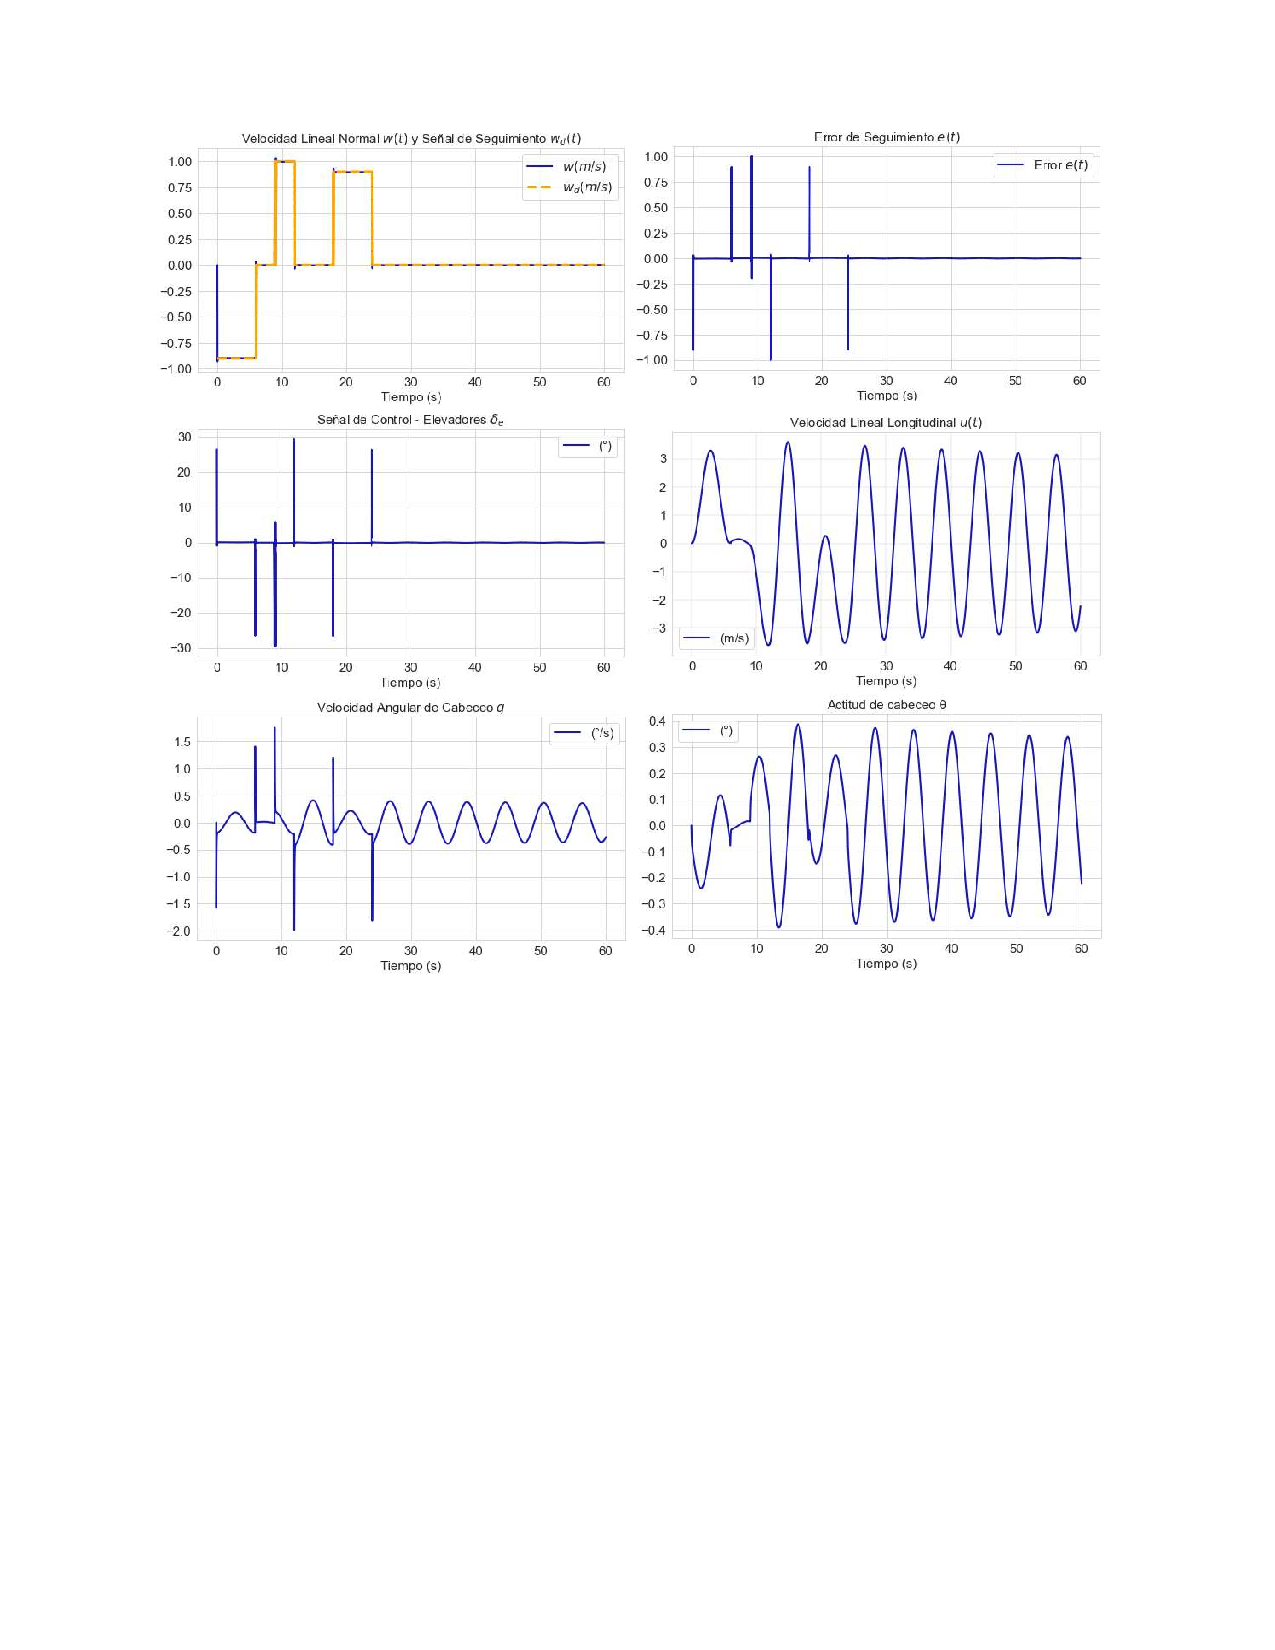
\includegraphics[scale=0.84]{Capitulo3/figs/Simulacion PID crucero_cropped.pdf}
    \caption{Simulación de Vuelo Crucero con Controlador PID}
    \label{Simulación de Vuelo Crucero con Controlador PID}
\end{figure}
\begin{table}[!h]
    \centering
    \begin{tabular}{|c|c|}
    \hline
    \multicolumn{2}{|c|}{Ganancias del Controlador PID Longitudinal}\\
    \hline
     Proporcional $k_p$ & $-25.150989512082$ \\
     Integral $k_i$ & $-715.814283072008$\\
     Derivativa $k_d$ & $0.0334264493487736$\\
     \hline
    \end{tabular}
    \caption{Ganancias del Controlador PID Longitudinal}
    \label{Ganancias del Controlador PID Longitudinal}
\end{table}

\textbf{Discusión de Resultados.} La Figura \ref{Simulación de Vuelo Crucero con Controlador PID} muestra los resultados del controlador PID para la dinámica longitudinal de EHEKATL BWB. De acuerdo con el movimiento oscilatorio en $q(t)$,$\theta(t)$ y $u(t)$ se observa un modo longitudinal fugoide con controles libres. Se propone la señal de seguimiento $w_d$, ver gráfica a). La función $w_d$ pretende imitar una perturbación inicial que obliga a la aeronave a ascender ligeramente (signo negativo) su altitud durante seis segundos. Logra recobrar brevemente su altitud constante cuando una segunda perturbación logra descenderla durante tres segundos. La aeronave recupera por un instante la altitud para volver a descender por una tercera y última perturbación,  para finalmente, mantenerse a altitud constante. 
%
En la gráfica b) se muestra el comportamiento del error de seguimiento en el tiempo. el error de seguimiento $e(t)$ crece tanto como la señal de seguimiento $w_d (t)$ lo demanda. Sin embargo, se observa una línea recta que vuelve rápidamente a cero. Esto quiere decir que el controlador PID está realizando una excelente tarea de seguimiento de acuerdo con las ganancias propuesta en \ref{Ganancias del Controlador PID Longitudinal}. 
%
La gráfica c) muestra la respuesta de los elevadores $\delta_e$ para cumplir con la trayectoria deseada de $w_d$. La respuesta de los elevadores es muy rápida y se encuentra en el rango de deflexión de $-30^\circ /+30 ^\circ$. 
%
La gráfica d) muestra la velocidad lineal longitudinal $u(t)$. Aquí, el valor nominal cero no representa un estado en reposo sino una velocidad uniforme o constante de $13.23m/s$. Entonces, el aumento o disminución de la velocidad $u(t)$ es una adición o substracción a esta velocidad constante. Se observa que la velocidad mantiene un movimiento oscilatorio debido a qué EHEKALTL BWB mantiene una leve oscilación de cabeceo con las entradas de control (elevadores) libres. Cuando $w_d$ demanda un cambio en la trayectoria generado por los elevadores $\delta_e$ Se percibe una respuesta de cambio en el movimiento oscilatario de $u(t)$. Cuando $w_d$ se mantiene en cero, $u(t)$ continua con el movimiento oscilatorio con elevadores fijos. 
%
La gráfica e) muestra la velocidad angular de cabeceo $q$. Se observa que responde en mismo sentido que la señal de seguimiento $w_d$. Mantiene un movimiento oscilatorio menor a $-0.5/0.5$ grados. 
%
Finalmente, la gráfica f) muestra la actitud de cabeceo $\theta$. La respuesta de $\theta$ es en el mismo sentido que $w_d$. Mantiene un suave movimiento oscilatorio entre $-0.4 / 0.4$ grados. 

\medskip

%%%%%%%%%%%%%%%%%%%%%%%%%%%%%%%%%%%%%%%%%%%%%%%%%%%%%%
\textbf{Simulación de Control PID para Giro Lateral}\\
Cuando una aeronave gira hacia un lado o hacia otro, se debe a la diferencia de sustentación que se genera en los extremos del ala debido a la deflexión de los alerones. 
Como se mencionó en el modelo dinámico, la deflexión del par de alerones en dirección opuestas genera un giro lateral. 
Aunque la dinámica lateral utiliza tanto los alerones como los timones, la contribución principal para un giro es mayormente de los alerones (alrededor de un $80\%$ dependiendo del tipo de aeronave y las condiciones de vuelo). Los timones suelen usarse para ajustar el rumbo o la dirección de la nariz y conseguir un movimiento lateral suave. 
Para la aplicación del control PID en EHEKATL BWB vamos a utilizar la señal de seguimiento $p_d$ para el control de la velocidad angular de alabeo $p$. 
Esta aplicación tiene como objetivo controlar el régimen de giro lateral, e integrando obtener la posición de traslación en el eje \textit{y} de acuerdo a una velocidad constante. 
el objetivo del controlador PID lateral de EHEKATL BWB es mantener giros sostenidos a distintas velocidades y regresar al vuelo a nivel del ala. 
Se asume a la aeronave a una  velocidad constante de $13.23 m/s$ para realizar un giro sostenido.
La ecuación \ref{PID lateral EHEKATL BWB} muestra la dinámica lateral de EHEKATL BWB en representación de espacio de estados para la simulación del sistema lineal invariante en el tiempo. 
\begin{equation}
\label{PID lateral EHEKATL BWB}
    \begin{bmatrix}
        \dot v \\
        \dot p \\
        \dot r \\
        \dot \phi
    \end{bmatrix}
    =
    \begin{bmatrix}
    -0.440144 & -0.263171 & -16.0681 & 9.81 \\
    -8.22254 & -22.4261 & 8.34045 & 0 \\
    2.0262 & 1.4176 &-1.72499 & 0 \\
    0 & 1 & 0 & 0 \\
    \end{bmatrix}
    \begin{bmatrix}
        v \\
        p \\
        r \\
        \phi
    \end{bmatrix}
    +
    \begin{bmatrix}
    2.882972 \\
    500.764 \\
    -18.97689 \\
    0\\
    \end{bmatrix}
    \delta_a
\end{equation}

El error de seguimiento se define como la señal deseada del régimen de alabeo $p_d(t)$ menos la señal real del régimen alabeo de EHEKATL BWB $p(t)$. 
\begin{equation}
    e(t) = p_d (t) - p(t)
\end{equation}
\begin{figure}[!h]
    \centering
    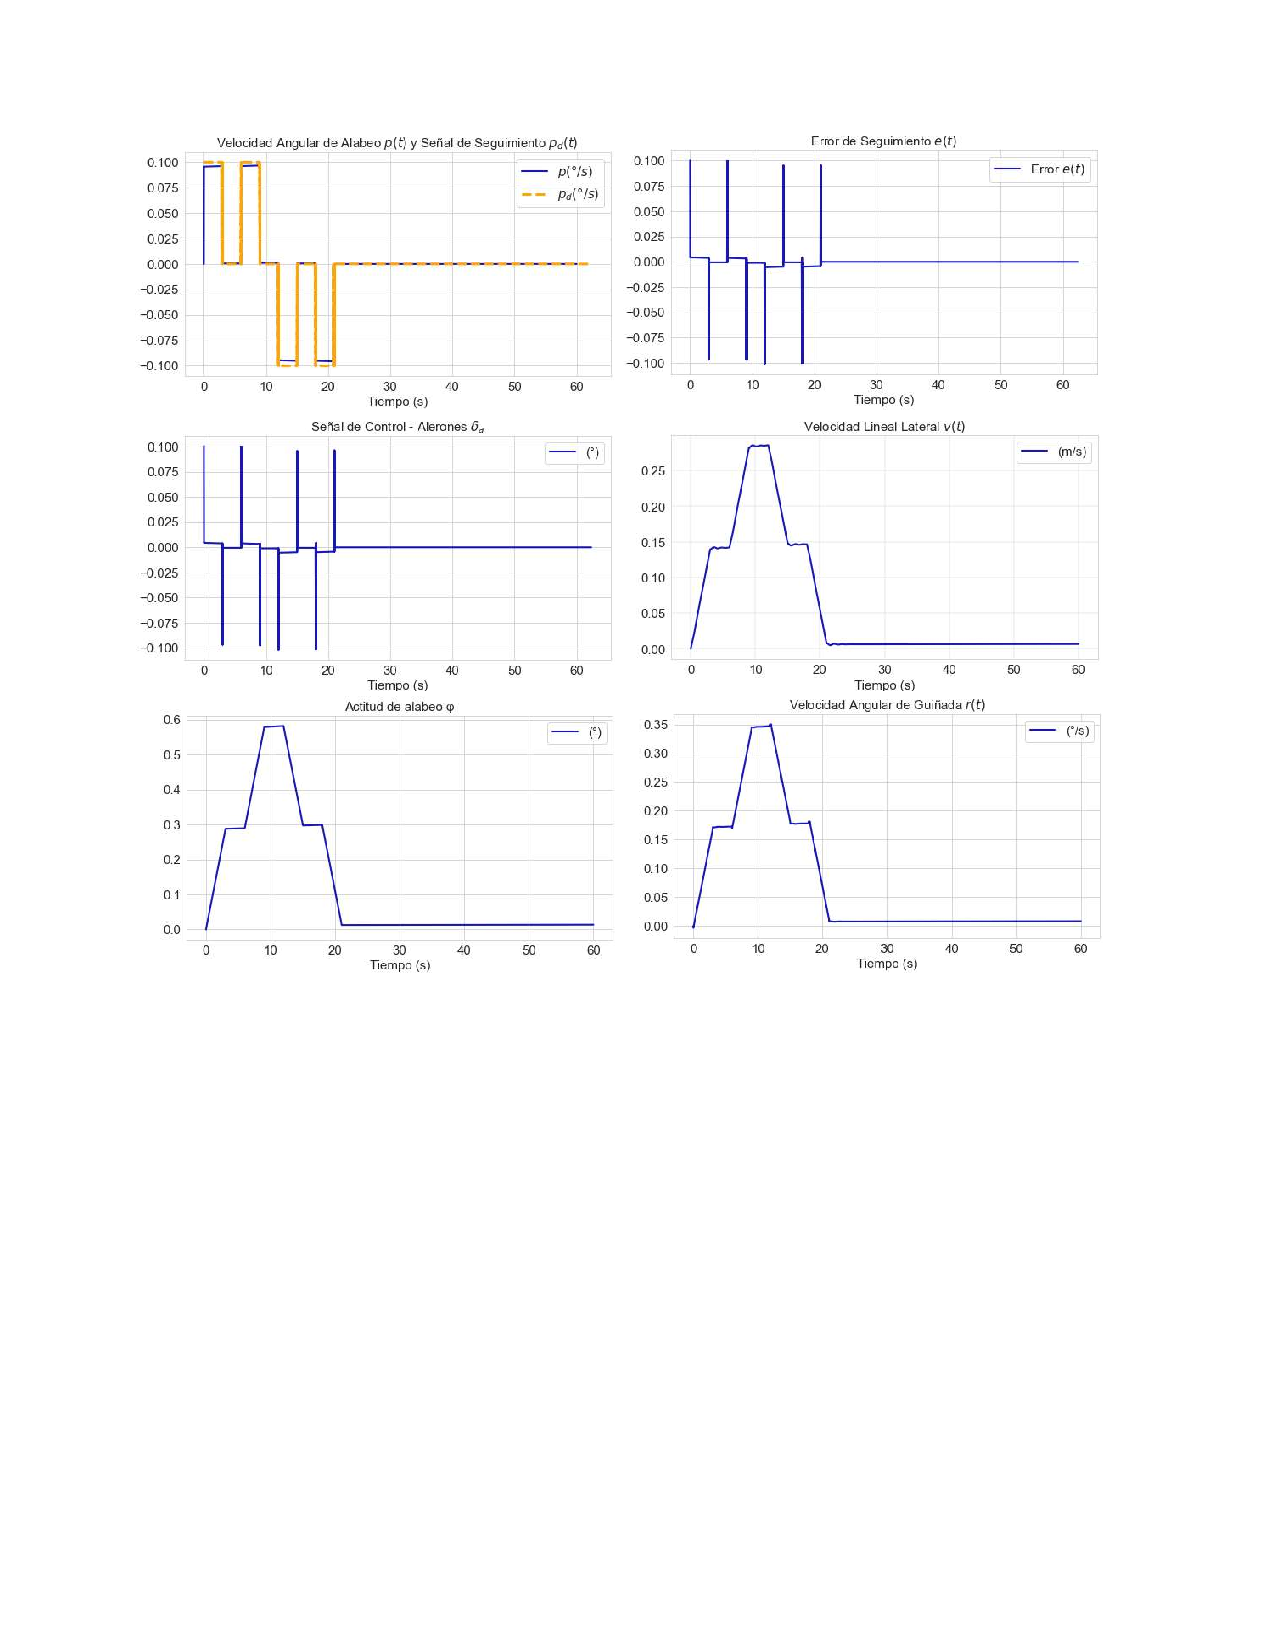
\includegraphics[scale=0.82]{Capitulo3/figs/Simulacion PID lateral_cropped.pdf}
    \caption{Simulación de Giro Lateral con Controlador PID}
    \label{Simulación de Giro Lateral con Controlador PID}
\end{figure}

Las ganancias del controlador PID lateral se muestran en la Tabla \ref{Ganancias del Controlador PID Lateral}.
\begin{table}[!h]
    \centering
    \begin{tabular}{|c|c|}
    \hline
    \multicolumn{2}{|c|}{Ganancias del Controlador PID}\\
    \hline
     Proporcional $k_p$ & $0.0393742116172623$ \\
     Integral $k_i$ & $1.39969270141192$\\
     Derivativa $k_d$ & $0$\\
     \hline
    \end{tabular}
    \caption{Ganancias del Controlador PID Lateral}
    \label{Ganancias del Controlador PID Lateral}
\end{table}

\textbf{Discusión de los Resultados.} En la Figura \ref{Simulación de Giro Lateral con Controlador PID} se observan los resultados de la simulación de giro sostenido de EHEKATL BWB.
%
De acuerdo con la gráfica a) la señal de seguimiento $p_d$ determina la régimen de giro (razón o velocidad). 
Aunque las ganancias del controlador PID lateral de la Tabla \ref{Ganancias del Controlador PID Lateral}  hacen que la señal de la razón de alabeo $p$ se aproxime rápido a la señal de seguimiento $p_d$, no logra alcanzarla, aunque se queda muy cerca. La señal de seguimiento $p_d$ pretende operar un giro hacia la derecha (valor positivo) en un régimen que incrementa a una razón de 0.1 grados por segundo durante los primeros segundos. Se mantiene en este giro sostenido para incrementar de nueva cuenta el régimen de alabeo a la misma razón de 0.1 grados por segundo antes de los primeros diez segundos. 
Se mantiene por un instante para después decrecer el régimen de giro logrado con una magnitud igual pero en sentido opuesto (valores negativos) respetando los mismos intervalos que las dos primeras señales de paso. Esta consideración hace que EHEKATL BWB recobre el vuelo a nivel del ala poco después de los viente segundos. 
%
La gráfica b) muestra el error de seguimiento $e(t)$. Aquí se observa que dado que la señal real de régimen de alabeo $p(t)$ no alcanza a la señal de seguimiento $p_d(t)$ el error de seguimiento $e(t)$ no alcanza el cero después de la señales de paso. Sin embargo, únicamente se distingue una línea recta o picos en $e(t)$ dada la rápida respuesta del controlador. 
%
La gráfica c) muestra la señal de control de los alerones $\delta_a$.  
La respuesta es rápida y dentro del rango de deflexión de $-0.1 / 0.1$ grados. 
%
La gráfica d) muestra la velocidad lineal lateral $v(t)$. Esta velocidad es la que determina el cambio de posición lineal lateral. De acuerdo con la primer señal de paso $p_d$, $v(t)$ logra una razón de desplazamiento de $0.14m/s$. Con la segunda señal de paso logra una razón de $0.28m/s$. La siguiente señal, ya con signo negativo, desciende a $v(t)$ de nueva cuenta a una razón de  $0.14m/s$ para finalmente con la última señal de paso recobrar el vuelo a nivel del ala con $v(t)$ igual a cero. 
%
La gráfica e) muestra la actitud de alabeo $\phi(t)$. con la primer señal de paso se logra una actitud de alabeo hacia al derecha de casi $0.3 ^\circ$. Con la segunda señal de paso la actitud de alabeo máxima de poco menos de $0.6 ^\circ$. 
%
Por último, la gráfica f) muestra la velocidad de guiñada $r(t)$ respecto al eje $z$. En la primer señal de paso se logra mantener un $r(t)$ de $17 ^\circ/s$ para con la segunda señal de paso lograr mantener un $r(t)$ máximo de $0.34 ^\circ/s$.


\bigskip

\textbf{Simulación de Control PID para Rumbo o Dirección}\\
El rumbo refiere a la dirección en la cual la nariz de la aeronave esta apuntando. 
Es una orientación que normalmente toma el eje $x$ con dirección hacia el norte como referencia inicial. 
Una aeronave estable en guiñada mantiene una dirección fija sin intervención del piloto. 
Mantener el rumbo es esencial para el seguimiento de la trayectoria de vuelo, por ejemplo.
Para el controlador direccional PID de EHEKATL BWB vamos a utilizar la señal de seguimiento $r_d$ para el control de la razón de guiñada $r$. 
El error de seguimiento se define como la señal deseada  $r_d(t)$ menos la velocidad de guiñada de EHEKATL BWB $r(t)$. 
\begin{equation}
    e(t) = r_d (t) - r(t)
\end{equation}
Se asumen las mismas condiciones de a una velocidad constante de $13.23 m/s$ para realizar las maniobras de guiñada, rumbo o dirección. 
En \ref{direcciooal lineal EHEKATL BWB} se muestra la dinámica direccional de EHEKATL BWB en representación en espacio de estados para las simulaciones del sistema lineal invariante en el tiempo. 
\begin{equation}
\label{direcciooal lineal EHEKATL BWB}
    \begin{bmatrix}
        \dot v \\
        \dot p \\
        \dot r \\
        \dot \phi
    \end{bmatrix}
    =
    \begin{bmatrix}
    -0.440144 & -0.263171 & -16.0681 & 9.81 \\
    -8.22254 & -22.4261 & 8.34045 & 0 \\
    2.0262 & 1.4176 &-1.72499 & 0 \\
    0 & 1 & 0 & 0 \\
    \end{bmatrix}
    \begin{bmatrix}
        v \\
        p \\
        r \\
        \phi
    \end{bmatrix}
    +
    \begin{bmatrix}
    4.206642e-13 \\
    -7.63414e-11 \\
    1.48159e-13 \\
    0 \\
    \end{bmatrix}
    \delta_r
\end{equation}

Las ganancias del controlador direccional PID de EHEKATL BWB se muestran en la Tabla \ref{Ganancias del Controlador PID direccional}. 
\begin{figure}[!h]
    \centering
    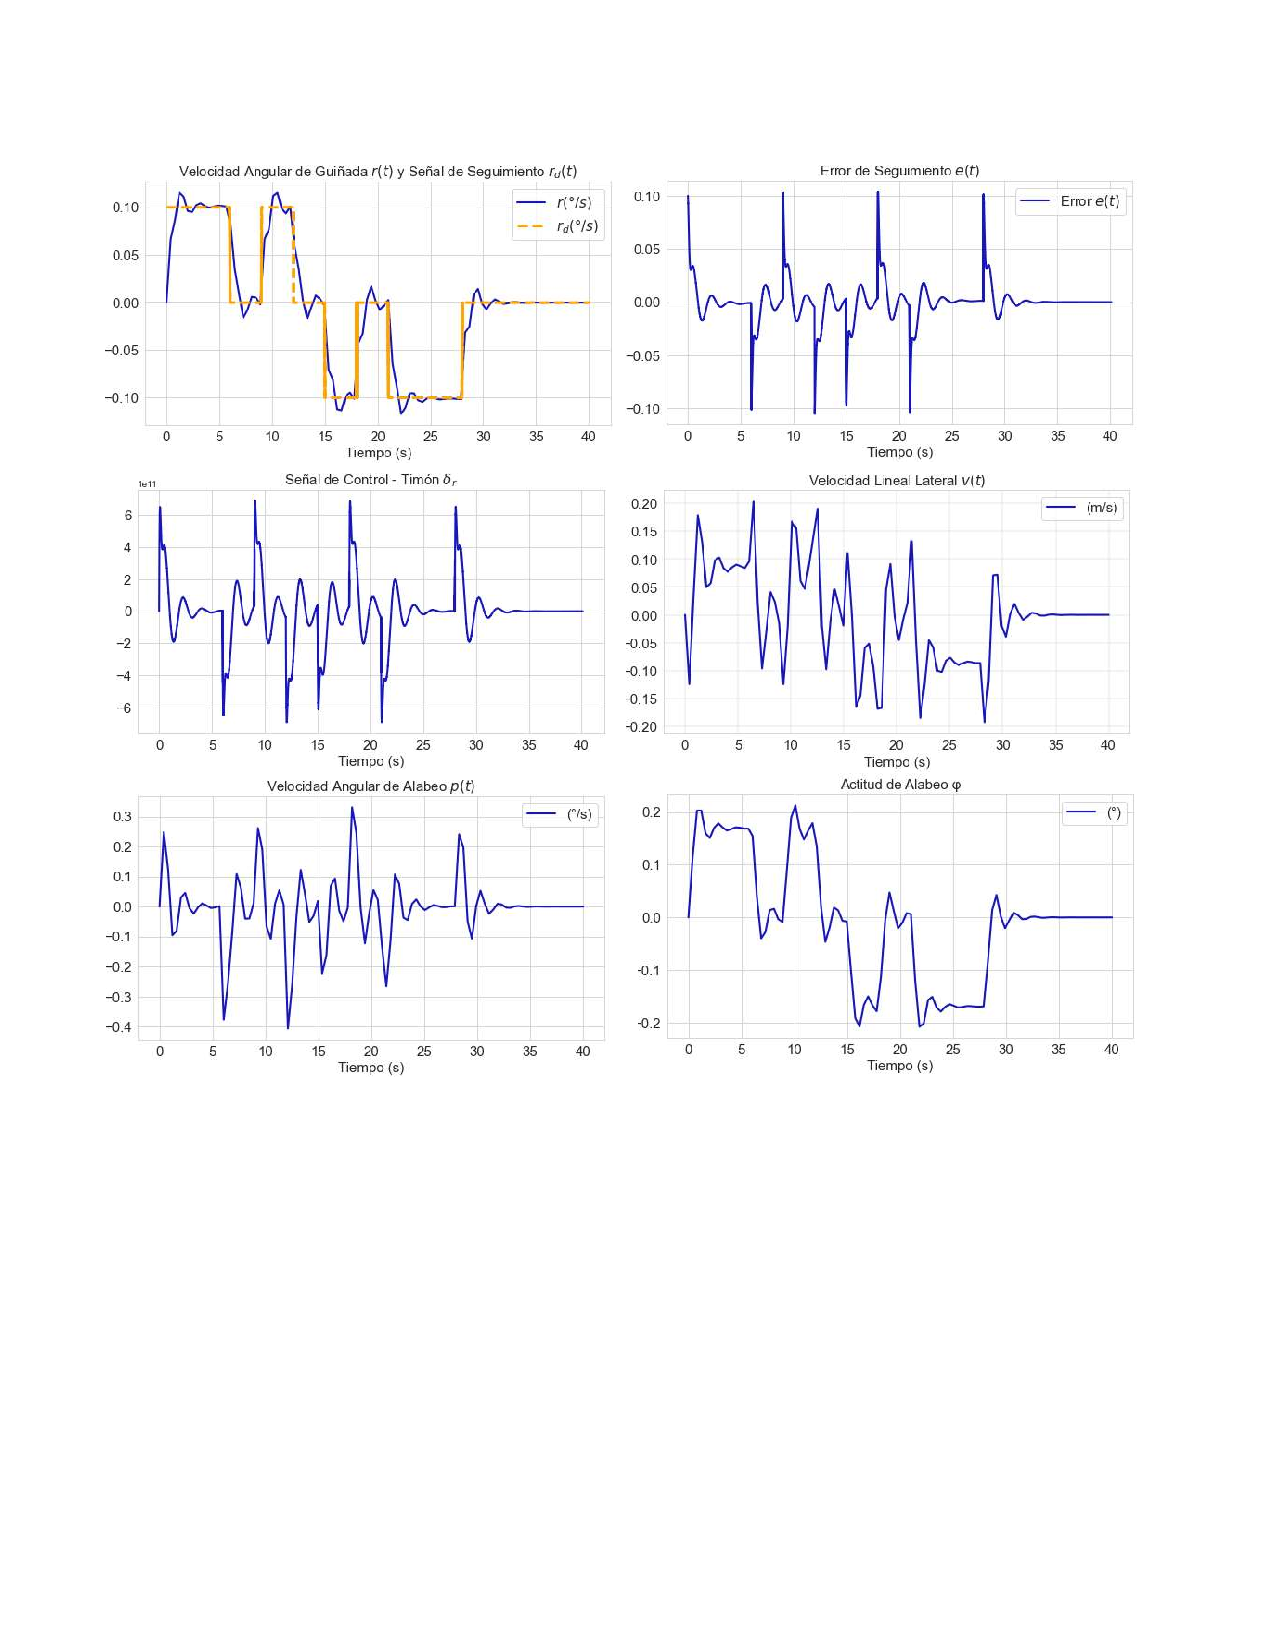
\includegraphics[scale=0.78]{Capitulo3/figs/Simulacion PID direccional_cropped.pdf}
    \caption{Simulación con Controlador PID Direccional}
    \label{Simulación de Giro Direccional con Controlador PID}
\end{figure}

\begin{table}[!h]
    \centering
    \begin{tabular}{|c|c|}
    \hline
    \multicolumn{2}{|c|}{Ganancias del Controlador PID}\\
    \hline
     Proporcional $k_p$ & $-1377938545499.12$ \\
     Integral $k_i$ & $-616745432554.002$\\
     Derivativa $k_d$ & $17142526949.4437$\\
     \hline
    \end{tabular}
    \caption{Ganancias del Controlador PID direccional}
    \label{Ganancias del Controlador PID direccional}
\end{table}

\textbf{Discusión de los Resultados.} La Figura \ref{Simulación de Giro Direccional con Controlador PID} muestra las simulaciones del controlador direccional PID para EHEKATL BWB. 
%
En la gráfica a) se percibe que el controlador PID direccional es menos robusto que los controladores PID longitudinal y lateral, mostrando oscilaciones para la aproximación de la señal $r(t)$ a la 
 señal de seguimiento $r_d(t)$. Sin embargo, este comportamiento también coincide con el sentido físico real, dado que el movimiento de guiñada es difícil de mantener por la simetría de la aeronave, y este movimiento oscilatorio alrededor de una trayectoria deseada en el rumbo o dirección es normal en aeronaves de ala fija. 
 %
 En la gráfica b) tenemos el error de seguimiento $e(t)$. A diferencia de los errores anteriores (dinámica longitudinal y lateral) aquí el $e(t)$ muestra un comportamiento oscilatorio y más suave. 
 %
 En la gráfica c) se observa la señal de control de los timones de dirección $\delta_r$. La señal de control es demasiado grande, se encuentra en el orden 1e11. Este resultado tan enorme de $\delta_r$ se debe a los valores tan pequeños que se obtuvieron en el vector de control $B$ de la ecuación \ref{direcciooal lineal EHEKATL BWB}. Por el mismo motivo las ganancias de la Tabla \ref{Ganancias del Controlador PID direccional} son tan grandes. 
 %
 En la gráfica d) se muestra la velocidad lineal lateral $v(t)$. Está gráfica va en el mismo sentido que la señal de seguimiento $r_d(t)$ pero con un rango de entre $-0.2 m/s$ y $0.2 m/s$. 
 %
 En la gráfica e) se observa la velocidad angular de alabeo $p(t)$, con una respuesta entre $-0.4m/s$ y $0.3m/s$. 
 %
 En la gráfica f) se muestra la actitud de alabeo $\phi(t)$. La respuesta coincide con la $r_d(t)$ en sentido, dónde positivo es dirrección a la derecha y negativo dirección a la izquierda. 

Los controladores PID diseñados para EHEKATL BWB pueden servir para aplicaciones similares a las que NASA tuvo con su aeronave de ala-integrada X-48 B/C, dónde se implementaron  controlador independientes PID para los momentos de cabeceo, alabeo y guiñada.
%
Durante el proceso de las simulaciones con los controladores PID se observó que ante nuevas señales de seguimiento (tipo senoidal o de paso pero con funciones más complejas) se necesita volver a sintonizar las ganancias. El re-ajuste de ganancias se debe principalmente a que las simulaciones son invariantes en el tiempo. Consideración importante que debe tenerse, dado que como la aplicación real de los controladores será para sistemas variantes en el tiempo, este ejercicio es una primera aproximación de control para las aplicaciones que se muestran en el capítulo de \textit{Simulaciones de vuelo de EHEKATL BWB}.  


%%%%%%%%%%%%%%%%%%%%%%%%%%%%%%%%%%%%%%%%%%

%%%%%%%%%%%%%
\section{Controlador Regulador Cuadrático Lineal}

El control Regulador Cuadrático Lineal\footnote{Linear Quadratic Regulator, o LQR por sus siglas en inglés} es una técnica avanzada de control utilizada en sistemas dinámicos lineales. 
%
Su objetivo es diseñar un controlador que minimice una función de costo cuadrática.
%
El control LQR se basa en dos aspectos clave: la formulación de una función de costo cuadrática que cuantifica el desempeño deseado del sistema y la resolución de la ecuación de Riccati para obtener las ganancias del controlador que minimizan esta función de costo. 
%
Recordando el capítulo de modelo dinámico, para el controlador LQR utilizamos el sistema de EHEKATL BWB en espacio de estados dada la forma $\dot x = Ax + Bu$, dónde $x$ es el vector de estados y $u$ es el vector de entradas de control. 

Se busca minimizar una función de costo cuadrática definida como:
\begin{equation}
    J = \int_0^{\infty} (x^T Qx + u^T Ru) dt
\end{equation}
dónde Q y R son las matrices de ponderación que determinan la importancia relativa de los estados y las entradas de control en el costo total.

La ecuación de Riccati en el controlador LQR es una ecuación matricial que se utiliza para encontrar la matriz de ganancias óptimas $K$ del controlador. La ecuación tiene la siguiente forma:
\begin{equation}
    A^T P + P A - P B R^{-1} B^T P + Q = 0
\end{equation}
dónde $A$ es la matriz de estados del sistema, $B$ es la matriz de entrada del sistema, $R$ es la matriz de ponderación de las entradas de control, $Q$ es la matriz de ponderación de los estados y $P$ es la matriz de solución que buscamos encontrar. 

Para aplicar el Control LQR, primero se debe tener el modelo del sistema en forma de espacio de estados con las matrices $A$ y $B$ definidas.
%
Posteriormente, se eligen las matrices de ponderación Q y R basadas en los objetivos de control. La elección de estas matrices afectará el desempeño del controlador. 
%
La ecuación de Riccati es una ecuación cuadrática en $P$, y puede ser resuelta de diversas maneras dependiendo de la naturaleza de las matrices involucradas. La solución puede ser analítica o numérica. En la práctica, es común utilizar herramientas computacionales para encontrar la solución numérica a la ecuación de Riccati. 
%
Se utiliza la librería de \textit{control.matlab} para Python para estimar $P$. La matriz $P$ contiene información sobre la forma en que los estados del sistema y las entradas de control están relacionados para minimizar la función de costo cuadrática. 
%
La solución de la ecuación de Riccati proporciona las ganancias óptimas para el controlador LQR, lo que significa que el controlador resultante minimizará la función de costo cuadrática.
%
Es importante destacar que la ecuación de Riccati puede tener múltiples soluciones. En la práctica, la solución dependerá de los objetivos específicos del diseño del controlador. 

\medskip

\textbf{Simulación de Control LQR para Vuelo Crucero}\\
Al igual que el controlador PID previo, LQR utiliza el sistema lineal con parámetros invariantes en el tiempo. 
%
\begin{figure}[!t]
    \centering
    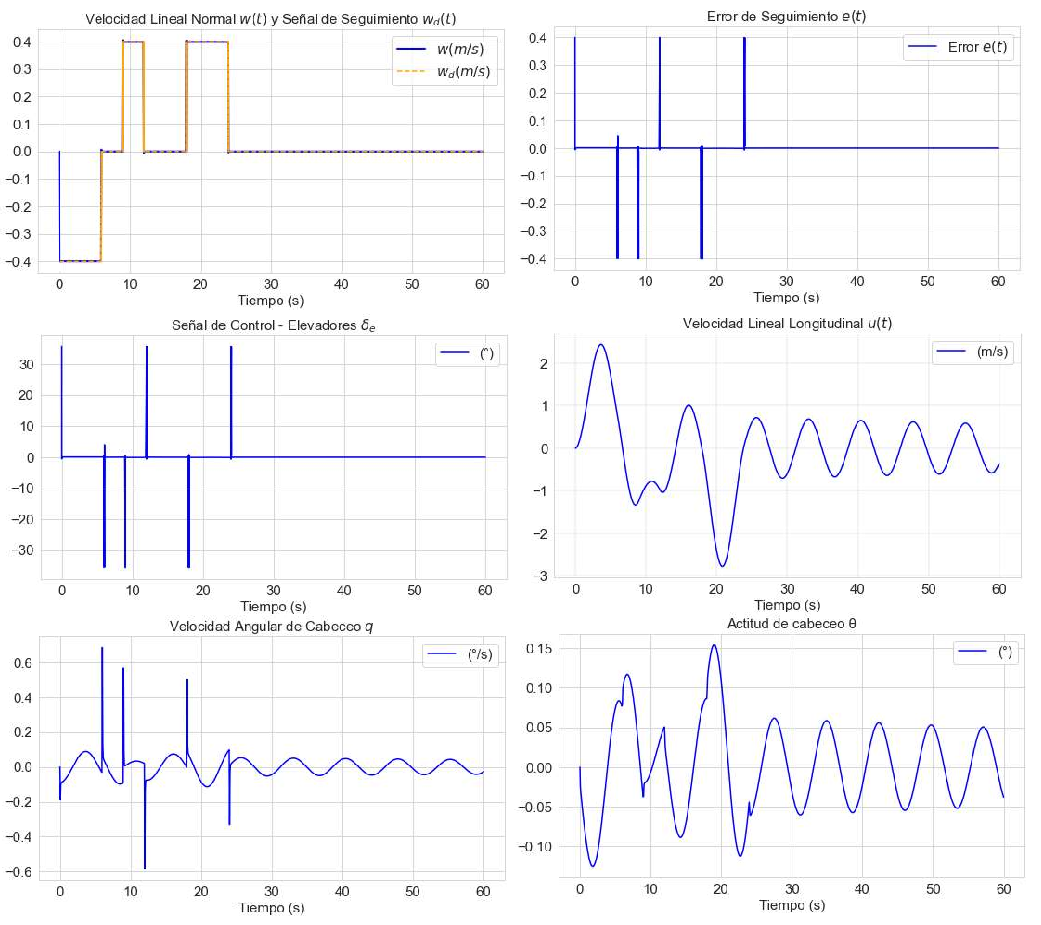
\includegraphics[scale=0.8]{Capitulo3/figs/LQR longitudinal.pdf}
    \caption{Simulación con Controlador LQR para Vuelo Crucero de EHKATL BWB}
    \label{Simulación con Controlador LQR para Vuelo Crucero de EHKATL BWB}
\end{figure}
Se muestra los valores del sistema A y B de EHEKATL BWB. 
\begin{equation}
    \begin{bmatrix}
    \dot u \\
    \dot w \\
    \dot q \\
    \dot \theta
    \end{bmatrix}
    =
    \begin{bmatrix}
    -0.0276445 & 0.467688 & 0 & -9.81 \\
    -1.1998 & -6.03618 & 13.3267 & 0 \\
    -6.70053e-07 &-4.84984 & -6.13596 & 0 \\
    0 & 0 & 1 & 0 \\ 
    \end{bmatrix}
        \begin{bmatrix}
    u \\
    w \\
    q \\
    \theta
    \end{bmatrix}
    +
    \begin{bmatrix}
    0.4311744\\
    -13.21339\\
    -27.35091\\
    0\\
    \end{bmatrix}
    \delta_{e}
\end{equation}

Se muestran los valores de las matrices de ponderación Q y R propuestos para la dinámica longitudinal. 
\begin{equation}
Q
=
\begin{bmatrix}
6 & 0 & 0 & 0 \\
0 & 18 & 0 & 0 \\
0 & 0 & 3 & 0 \\
0 & 0 & 0 & 0.1
\end{bmatrix} 
\quad
    R
    =
    \begin{bmatrix}
    0 & 0 & 0 & 0 \\
    0 & 0.001 & 0 & 0  \\
    0 & 0 & 0 & 0 \\
    0 & 0 & 0 & 0 \\
    \end{bmatrix}
\end{equation}

Y de acuerdo con el sistema dinámico de EHEKATL BWB para un instante en el tiempo (invariante en el tiempo) descrito por las matrices A y B, y nuestra ponderación en las matrices Q y R, calculamos de forma numérica a través de la librería de $control.matlab$ en Python las ganancias de la matriz de controlador $k$.
\begin{equation}
    K
    =
    \begin{bmatrix}
    48.9349891 & -89.19222159 & -41.54753902 & -691.77049282 \\
    \end{bmatrix}
\end{equation}
La figura \ref{Simulación con Controlador LQR para Vuelo Crucero de EHKATL BWB} muestra los resultados obtenidos después de aplicar al controlador LQR la misma señal de referencia $w_d$ que aplicamos en el controlador PID. 
%
Los resultados obtenidos con el controlador LQR son muy similares a los obtenidos con el controlador PID, que porsupuesto era de esperarse dada la misma señal de seguimiento $w_d$ y mimos valores en A y B. 

\medskip

%%%%%%%%%%%%%%%%%%
\textbf{Simulación de Control LQR para Giro Lateral}\\
Se utiliza el sistema dinámico lineal invariante en el tiempo para dinámica lateral, ver ecuación \ref{lateral lineal LQR EHEKATL BWB}. 
La figura \ref{Simulación con Control LQR para la dinámica lateral de EHEKATL BWB} muestra las simulaciones con el controlador LQR para EHEKATL BWB suponiendo un giro sostenido lateral a velocidad constante. 
\begin{figure}[!h]
    \centering
    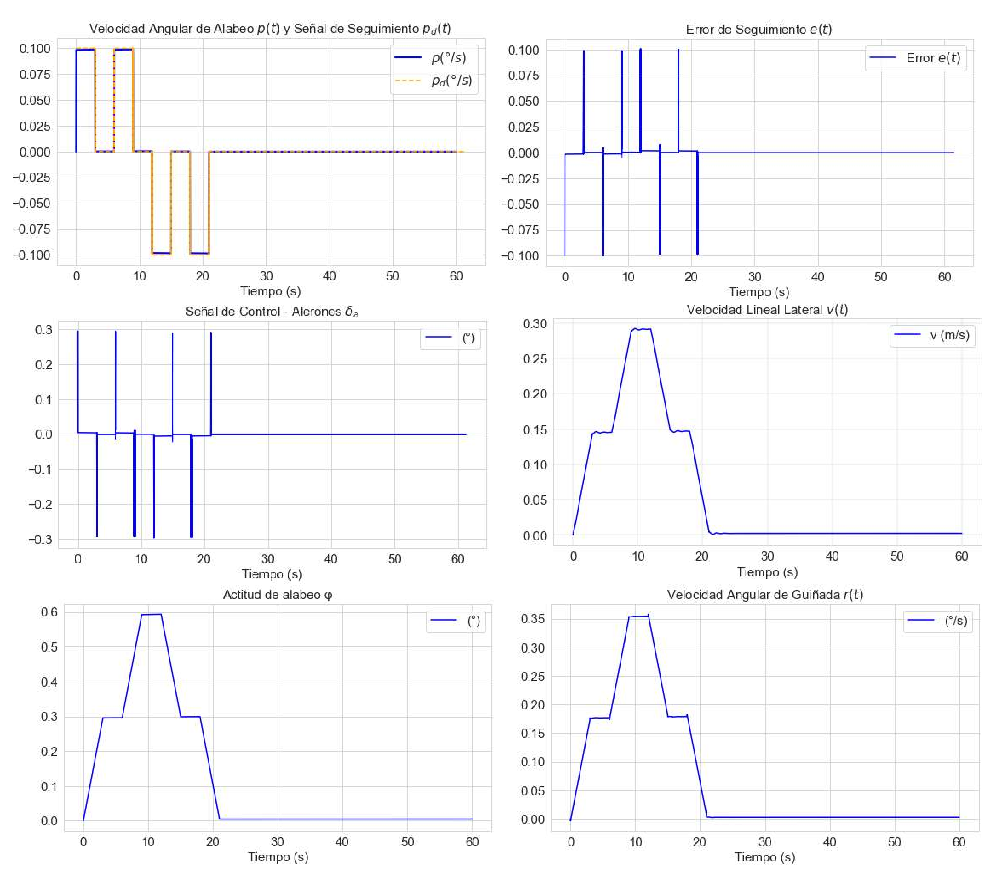
\includegraphics[scale=0.75]{Capitulo3/figs/LQR lateral.pdf}
    \caption{Simulación con Control LQR para la dinámica lateral de EHEKATL BWB}
    \label{Simulación con Control LQR para la dinámica lateral de EHEKATL BWB}
\end{figure}
\begin{equation}
\label{lateral lineal LQR EHEKATL BWB}
    \begin{bmatrix}
        \dot v \\
        \dot p \\
        \dot r \\
        \dot \phi
    \end{bmatrix}
    =
    \begin{bmatrix}
    -0.440144 & -0.263171 & -16.0681 & 9.81 \\
    -8.22254 & -22.4261 & 8.34045 & 0 \\
    2.0262 & 1.4176 &-1.72499 & 0 \\
    0 & 1 & 0 & 0 \\
    \end{bmatrix}
    \begin{bmatrix}
        v \\
        p \\
        r \\
        \phi
    \end{bmatrix}
    +
    \begin{bmatrix}
    2.882972 \\
    500.764 \\
    -18.97689 \\
    0\\
    \end{bmatrix}
    \delta_a
\end{equation}
Se propone la ponderación de las ganancias Q y R. 
\begin{equation}
Q
=
\begin{bmatrix}
3 & 0 & 0 & 0 \\
0 & 9 & 0 & 0 \\
0 & 0 & 9 & 0 \\
0 & 0 & 0 & 3
\end{bmatrix} 
\quad
R
=
\begin{bmatrix}
0 & 0 & 0 & 0 \\
0 & 1 & 0 & 0  \\
 0 & 0 & 0 & 0 \\
0 & 0 & 0 & 0 \\
\end{bmatrix}
\end{equation}

y de acuerdo con la parametrización de A,B,Q,R se obtienen de mediante solución de métodos numéricos las ganancias del controlador $k$.
\begin{equation}
    K
    =
    \begin{bmatrix}
     0.11366923 &  2.95176288 & -0.16714788 &   2.67770629\\
    \end{bmatrix}
\end{equation}
La propuesta de ponderación de importancia relativa propuesta por un servidor en las matrices Q y R resultó en excelente resultados para controlar la dinámica lateral mediante LQR. 

%%%%%%%%%%%%%%%%%%
\section{Códigos Python}
\label{a codigos python}
Los códigos desarrollados en este proyecto de tesis se comparten en la cuenta personal de Git-Hub del autor de la tesis. Aquí el acceso: 
\href{https://github.com/Galexs-Aerospace/Aircraft-Design-and-Control.git}{Aircraft Design and Control} o si prefiere: https://github.com/Galexs-Aerospace/Aircraft-Design-and-Control.git


